%---------------------------------------------SCP41 (Con y Sin B)
\begin{figure}[htp] 
    \centering
    \subfloat[]{%
        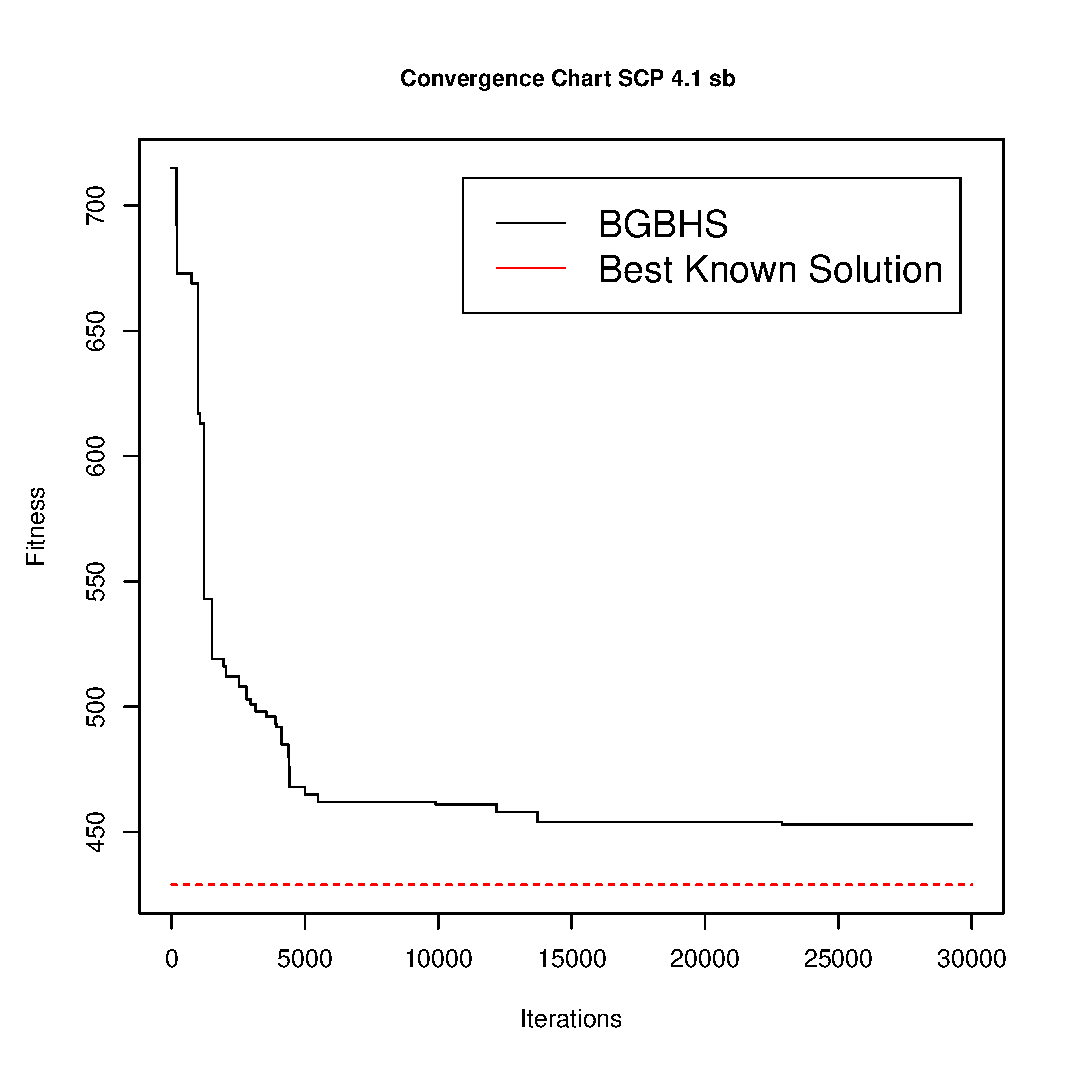
\includegraphics[width=0.45\textwidth]{Resultados/scp41_sb.eps}%
        \label{fig:b}%
        }%    
    \hfill%
    \subfloat[]{%
        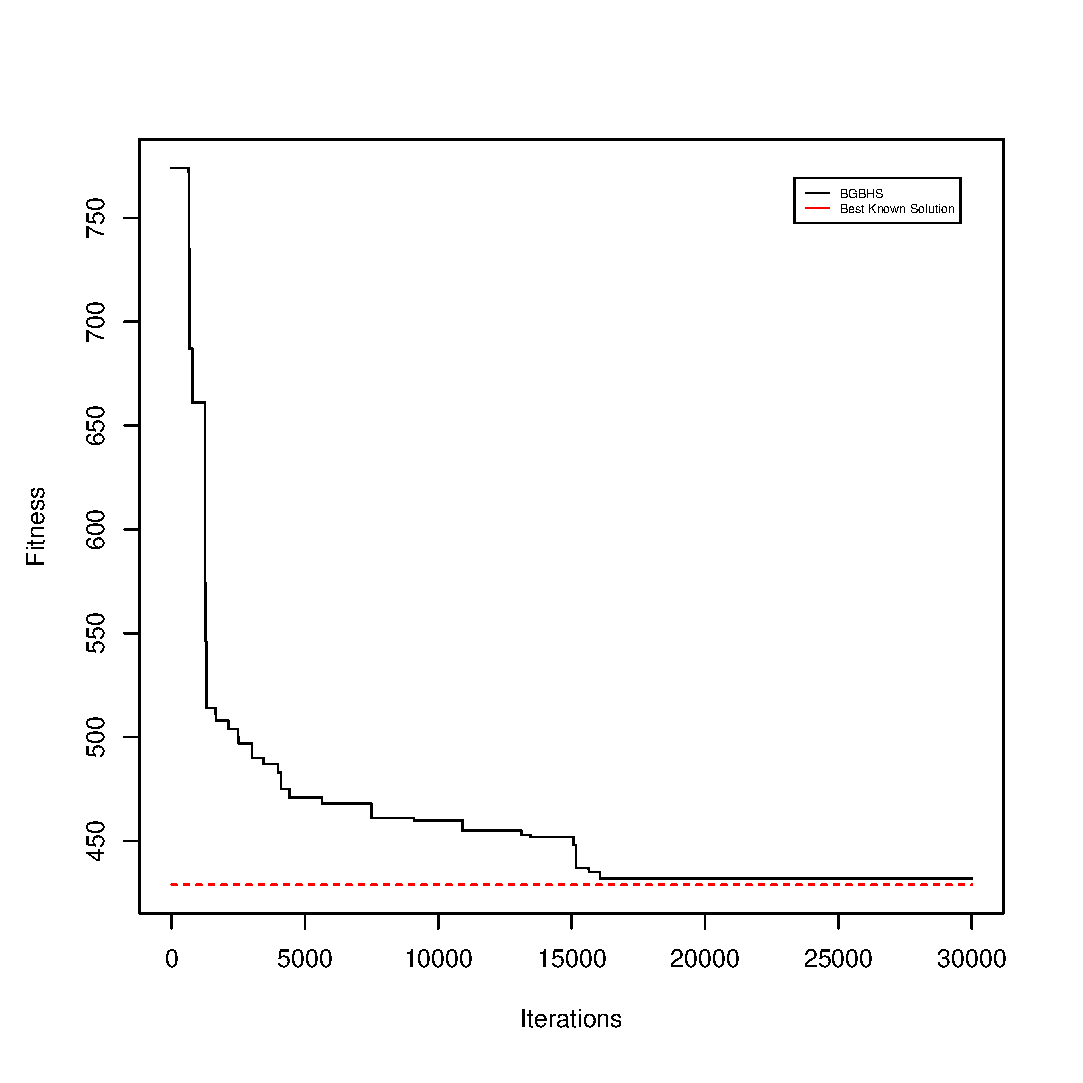
\includegraphics[width=0.45\textwidth]{Resultados/scp41.eps}%
        \label{fig:a}%
        }%
        \caption{Parameter $p$ fixed versus adaptive $p$ parameter for SCP41.}
\end{figure}



%---------------------------------------------SCP41
%%!htb
%\begin{figure}[]
%\centering
%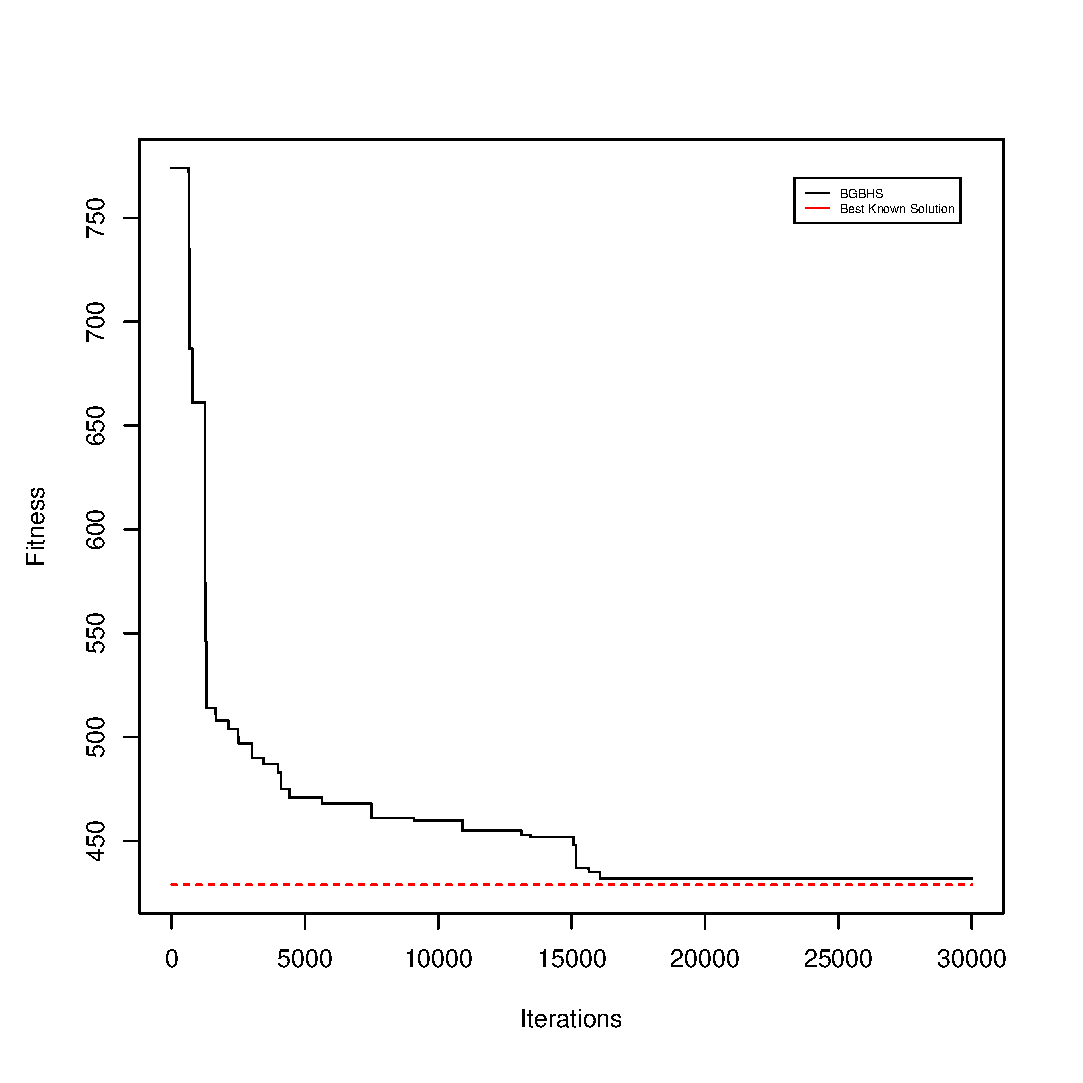
\includegraphics[scale=.45]{Resultados/scp41.eps}
%\caption{Instance 4.1.}
%\label{fig:Instance.4.1}
%\end{figure}
%%!htb
%\begin{figure}[]
%\centering
%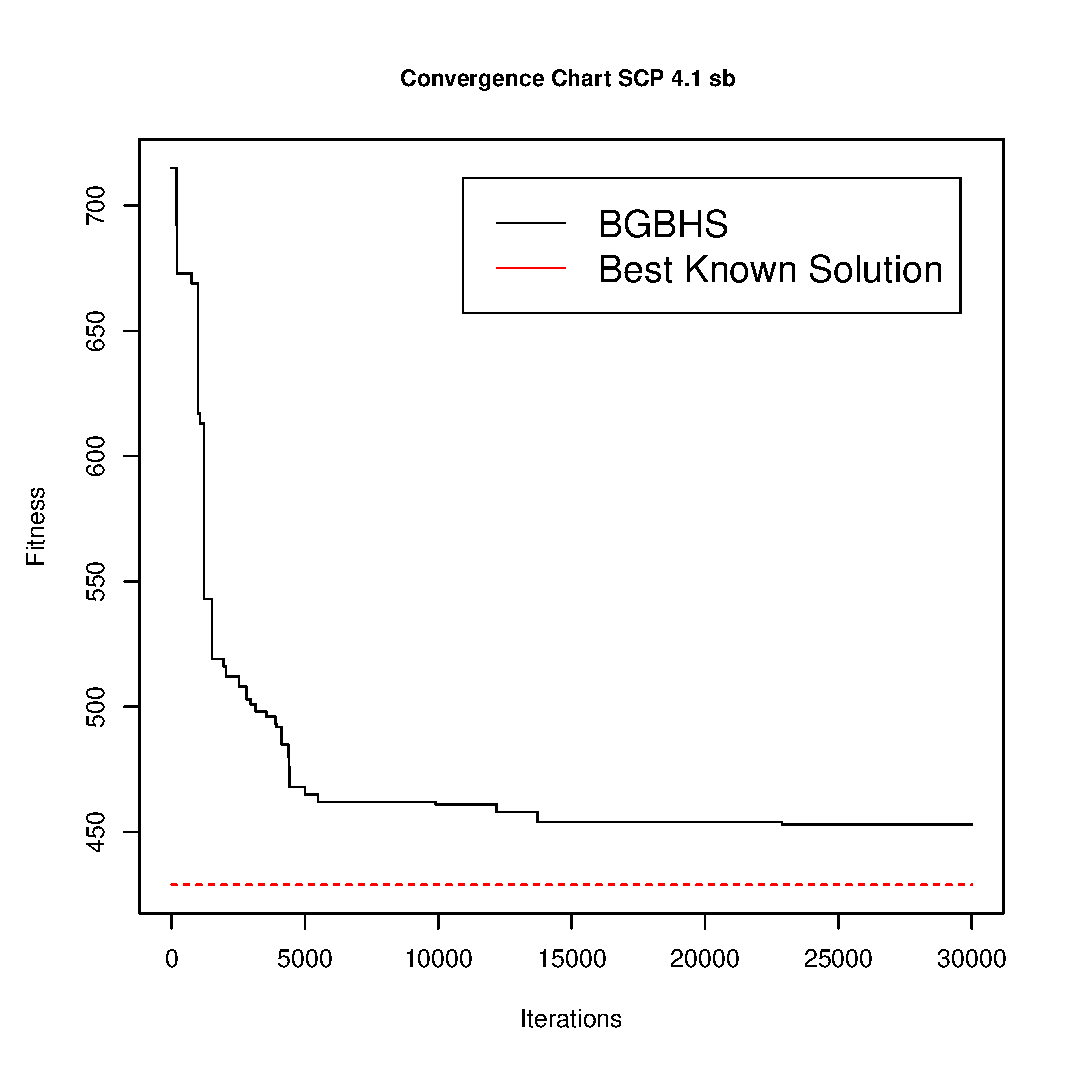
\includegraphics[scale=.45]{Resultados/scp41_sb.eps}
%\caption{Instance 4.1 SB.}
%\label{fig:Instance.4.1.SB}
%\end{figure}

%---------------------------------------------SCP42
\begin{figure}[]
\centering
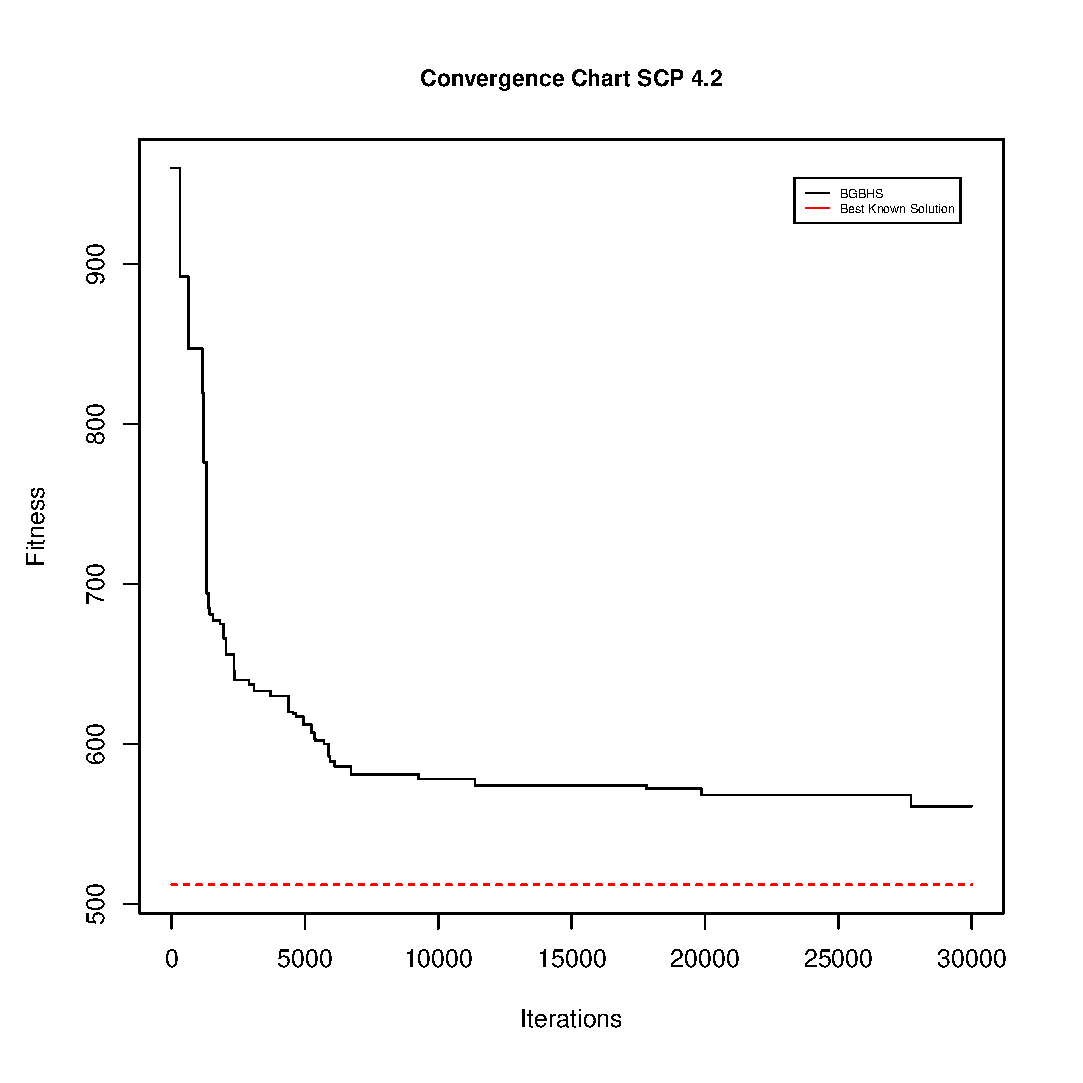
\includegraphics[scale=.45]{Resultados/scp42.eps}
\caption{Instance 4.2.}
\label{fig:Instance.4.2}
\end{figure}

%Limpieza de objetos, para liberar memoria.
\clearpage

%---------------------------------------------SCP43
\begin{figure}[]
\centering
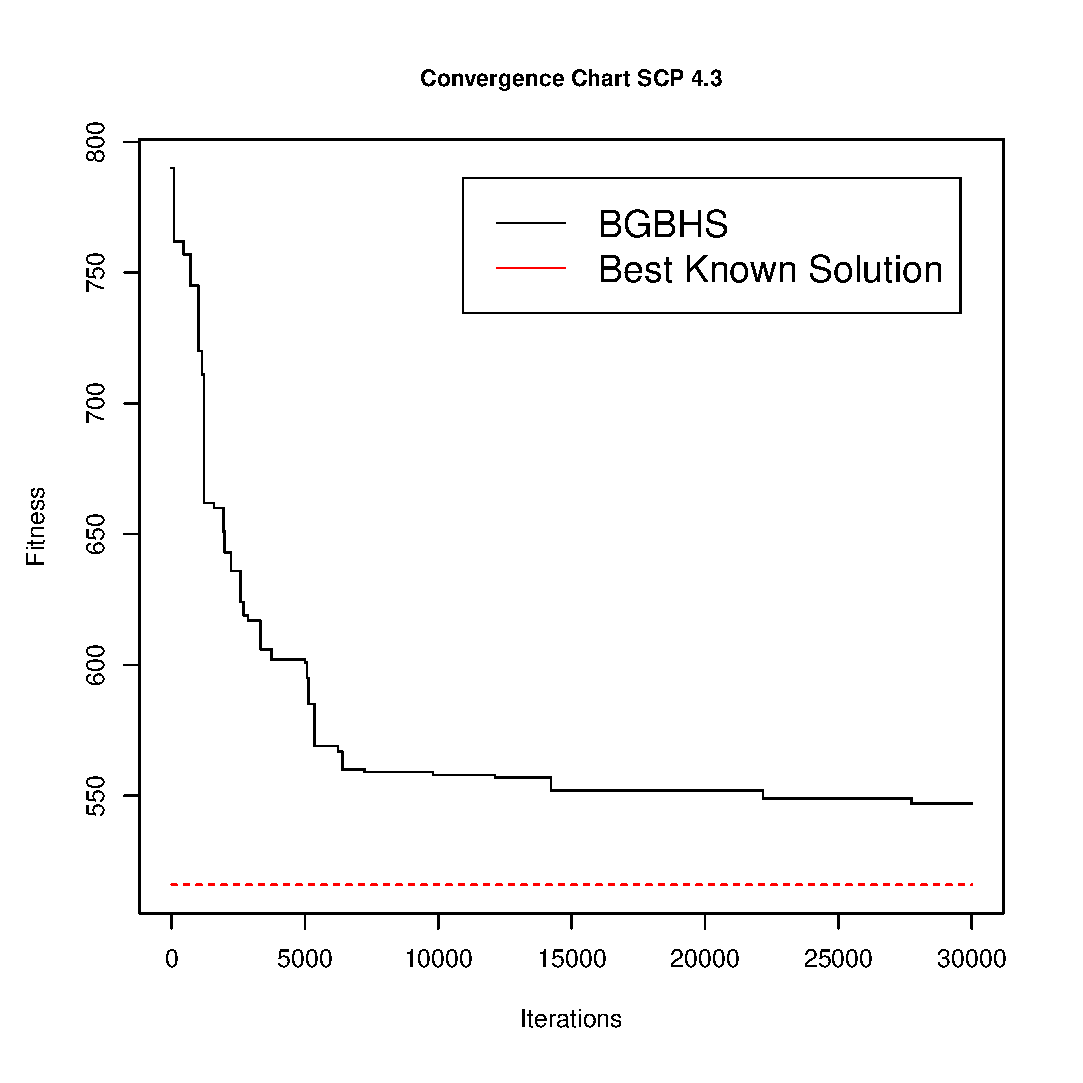
\includegraphics[scale=.5]{Resultados/scp43.eps}
\caption{Instance 4.3.}
\label{fig:Instance.4.3}
\end{figure}

%---------------------------------------------SCP44
\begin{figure}[]
\centering
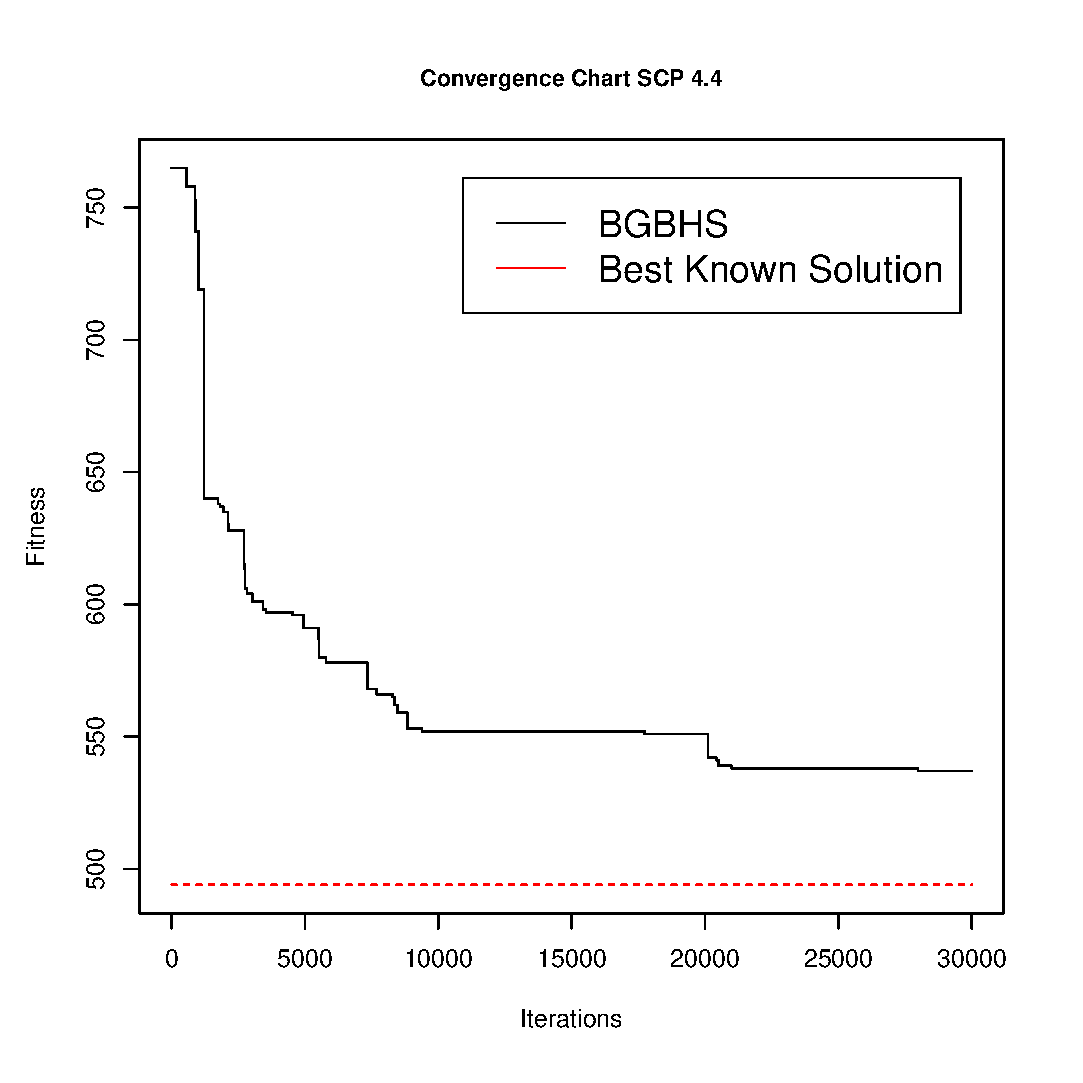
\includegraphics[scale=.45]{Resultados/scp44.eps}
\caption{Instance 4.4.}
\label{fig:Instance.4.4}
\end{figure}

%---------------------------------------------SCP45
\begin{figure}[]
\centering
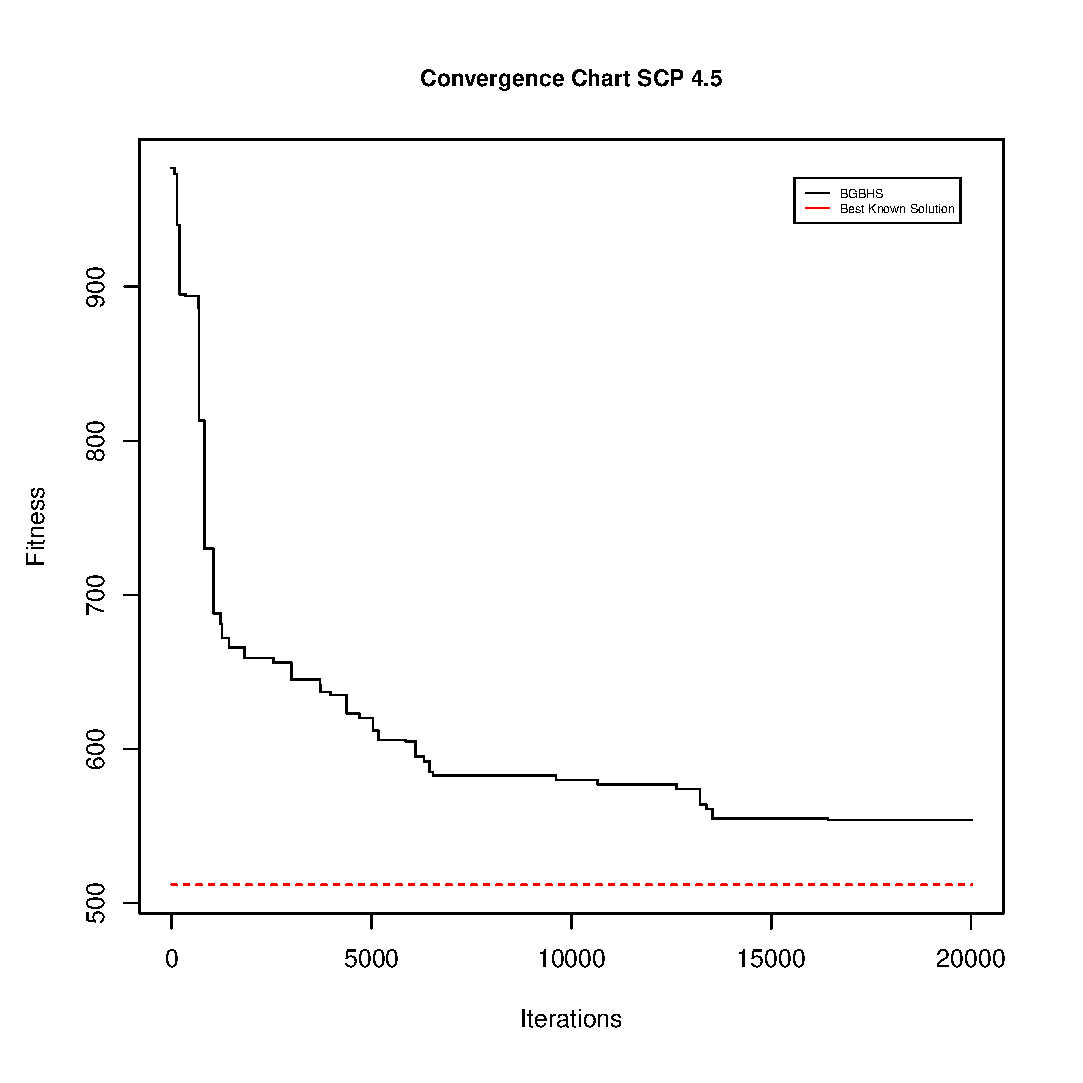
\includegraphics[scale=.45]{Resultados/scp45.eps}
\caption{Instance 4.5.}
\label{fig:Instance.4.5}
\end{figure}

%---------------------------------------------SCP46
\begin{figure}[]
\centering
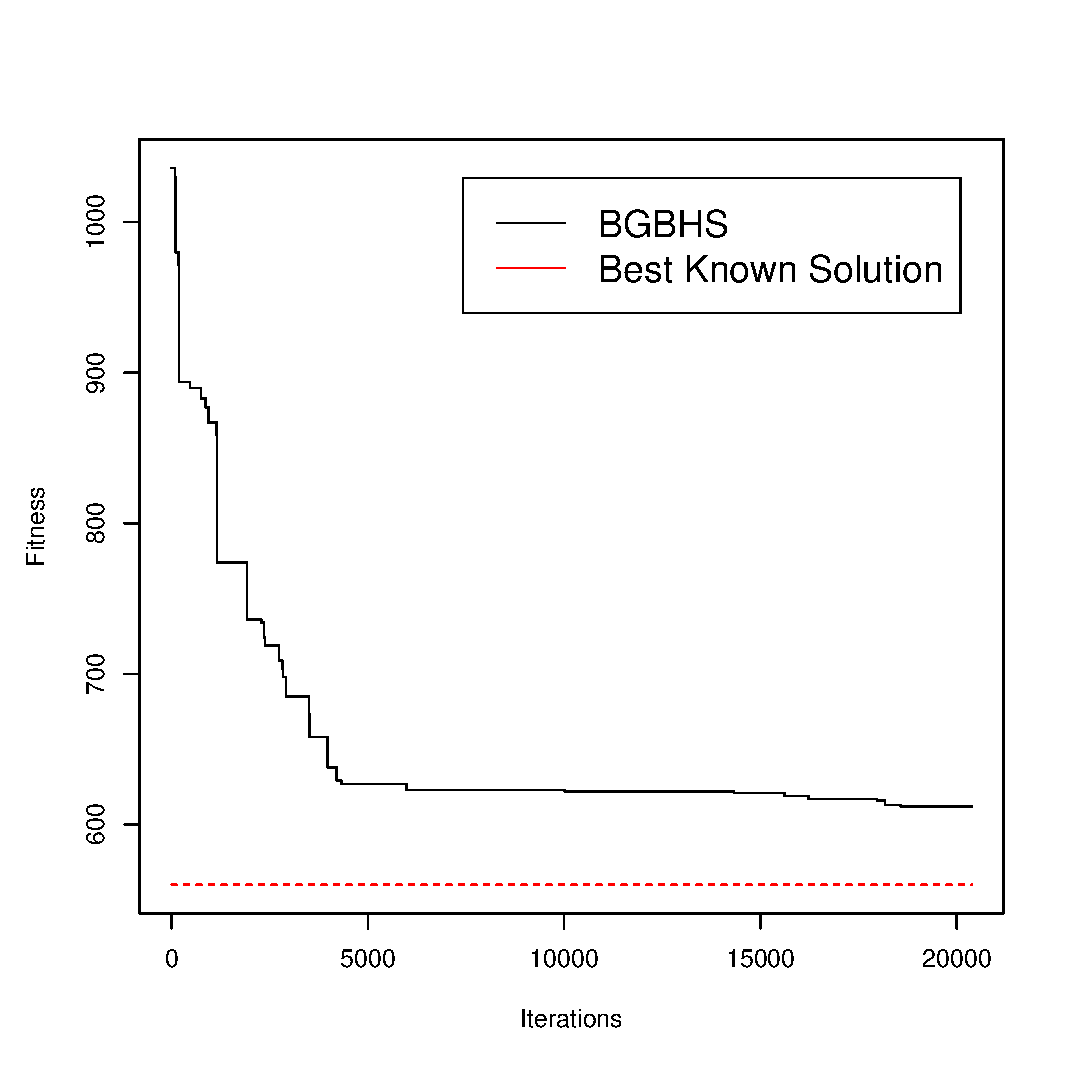
\includegraphics[scale=.45]{Resultados/scp46.eps}
\caption{Instance 4.6.}
\label{fig:Instance.4.6}
\end{figure}

%---------------------------------------------SCP47
\begin{figure}[]
\centering
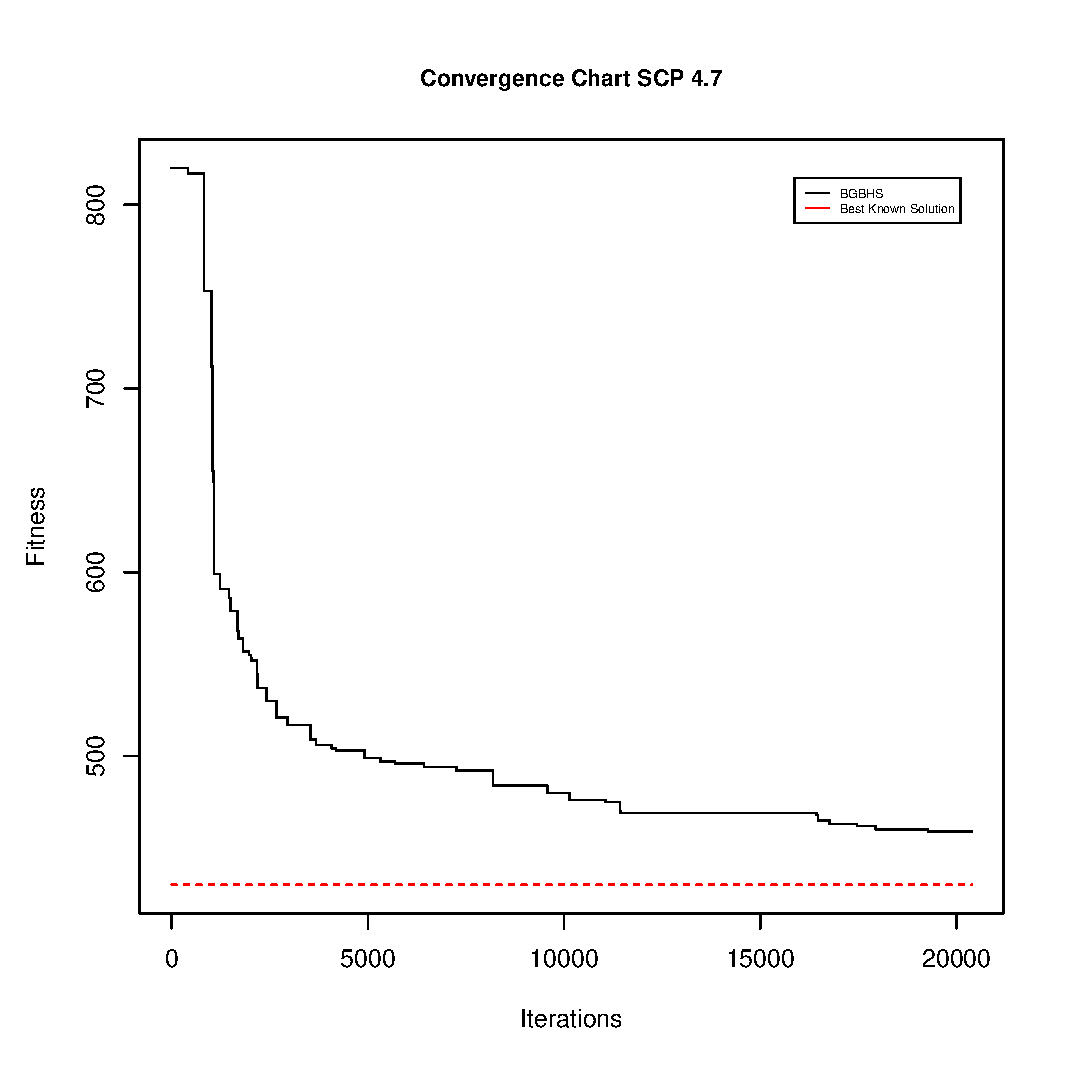
\includegraphics[scale=.45]{Resultados/scp47.eps}
\caption{Instance 4.7.}
\label{fig:Instance.4.7}
\end{figure}

%---------------------------------------------SCP48
\begin{figure}[]
\centering
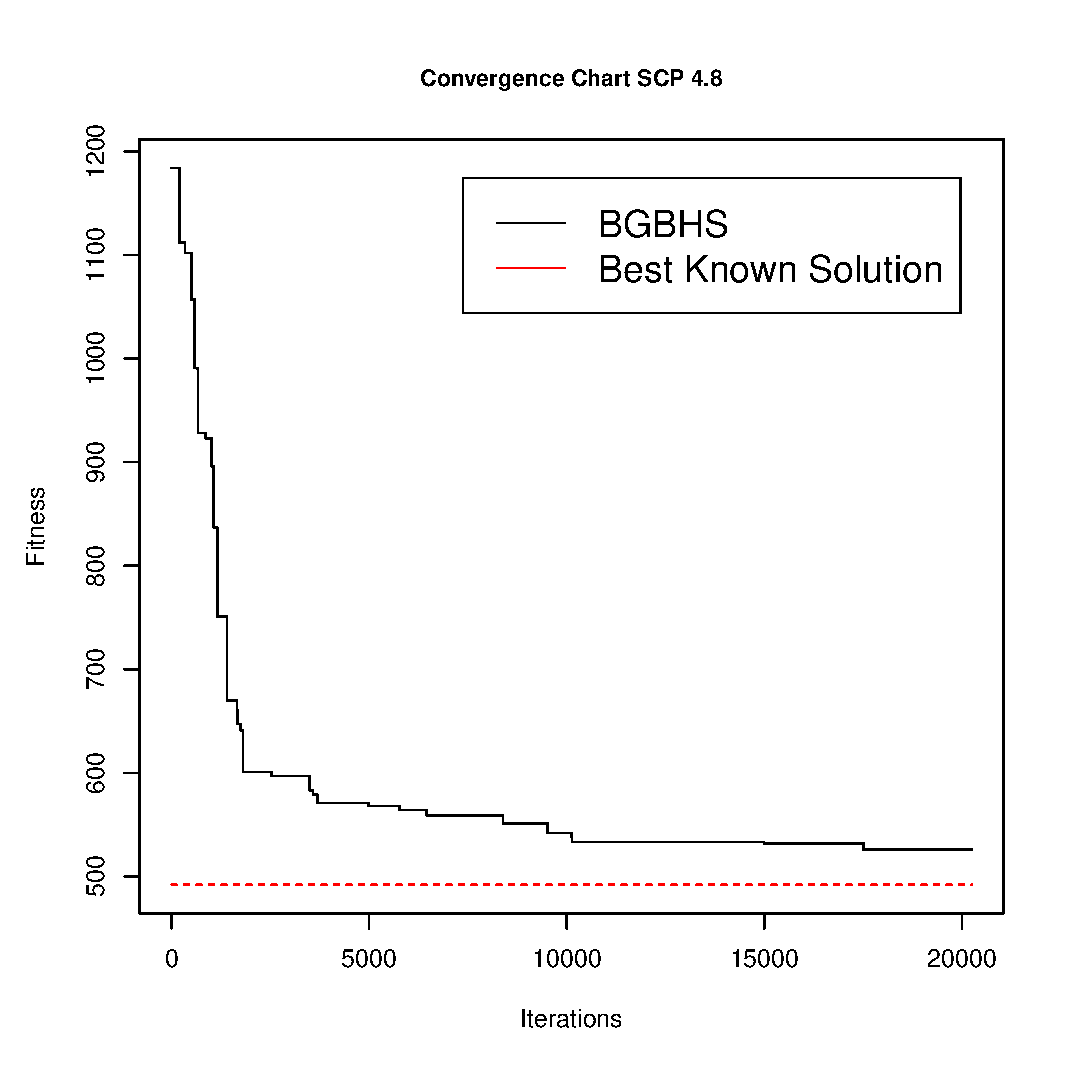
\includegraphics[scale=.45]{Resultados/scp48.eps}
\caption{Instance 4.8.}
\label{fig:Instance.4.8}
\end{figure}

%---------------------------------------------SCP49
\begin{figure}[]
\centering
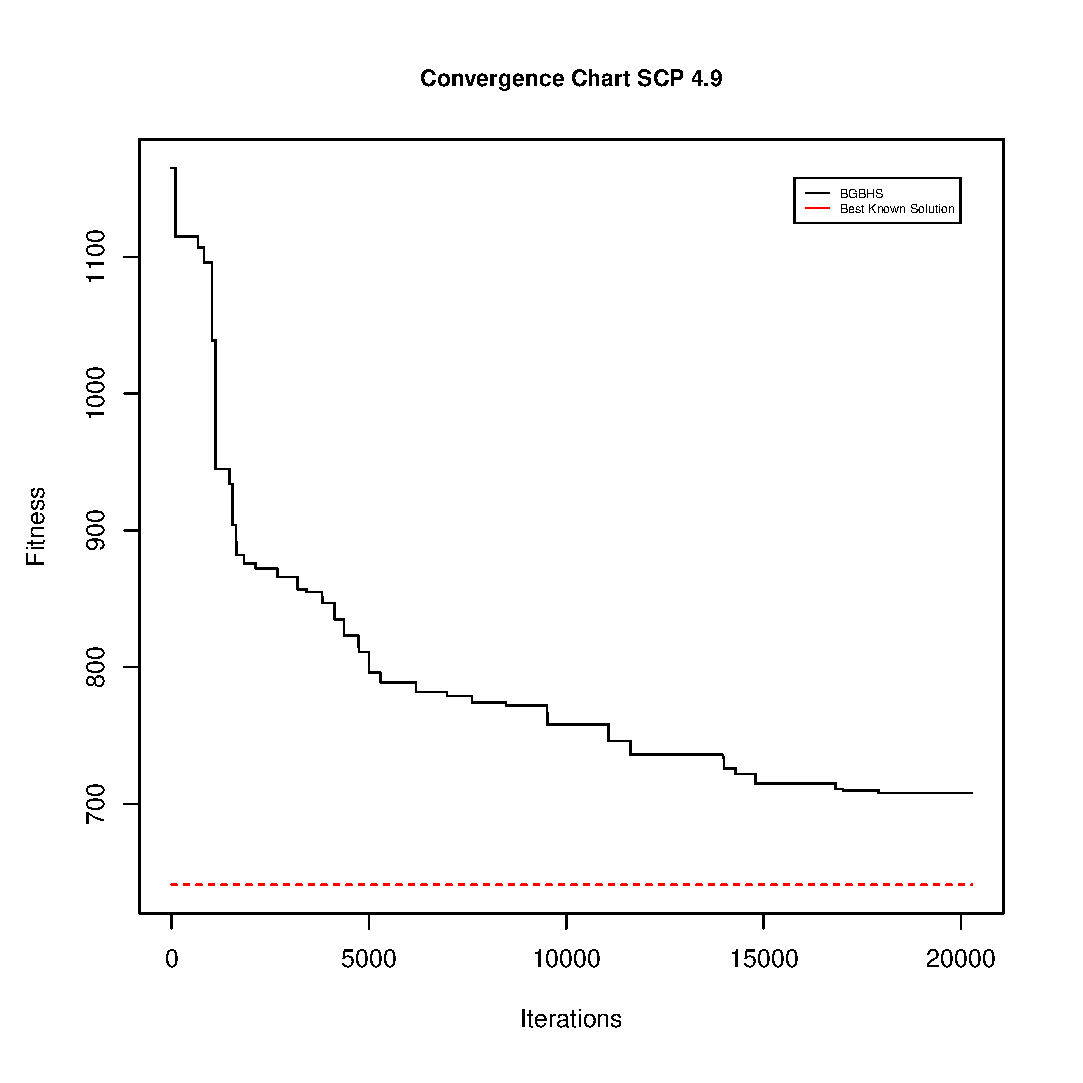
\includegraphics[scale=.45]{Resultados/scp49.eps}
\caption{Instance 4.9.}
\label{fig:Instance.4.9}
\end{figure}

%---------------------------------------------SCP410
\begin{figure}[]
\centering
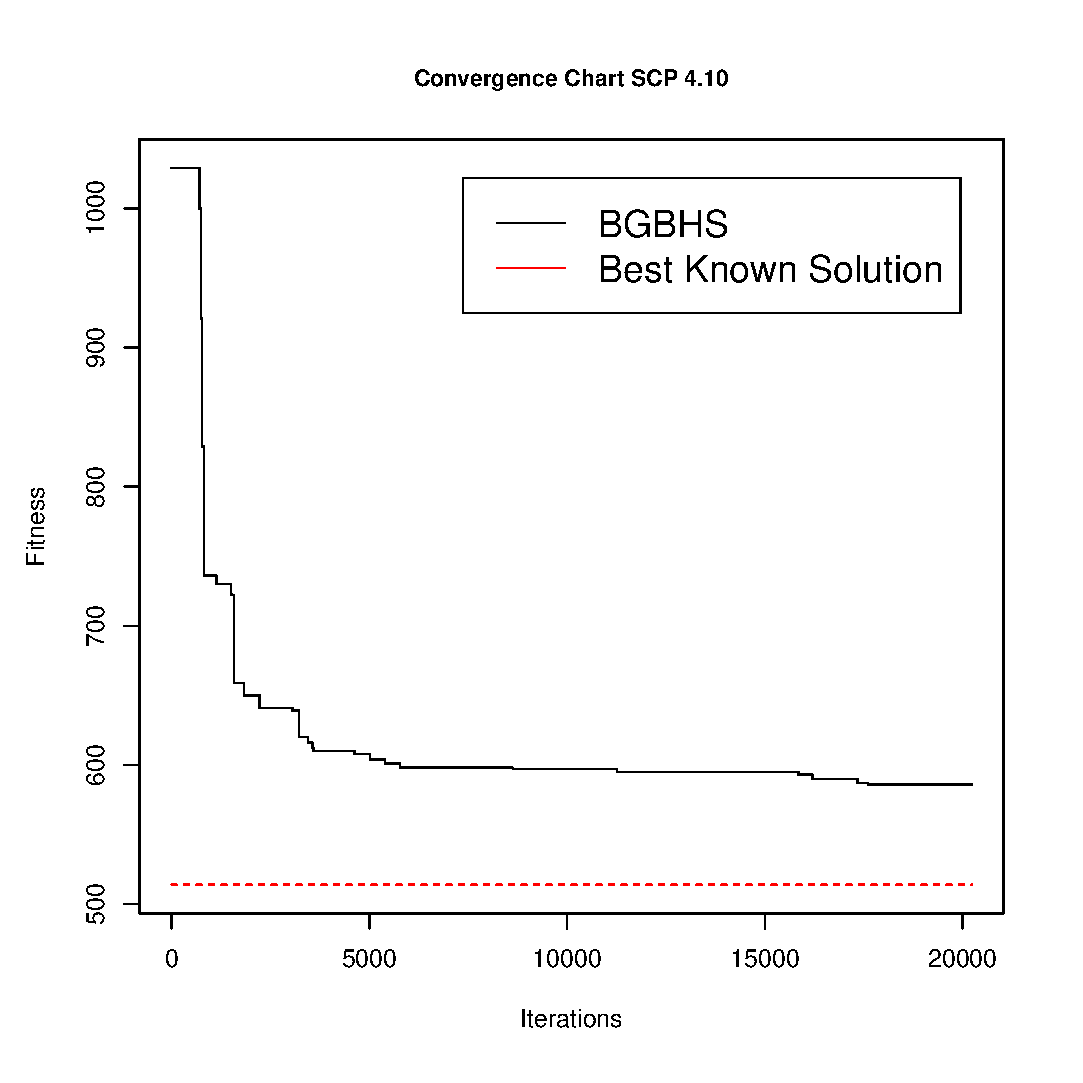
\includegraphics[scale=.45]{Resultados/scp410.eps}
\caption{Instance 4.10.}
\label{fig:Instance.4.10}
\end{figure}

%---------------------------------------------SCP51
\begin{figure}[htp] 
    \centering
    \subfloat[]{%
        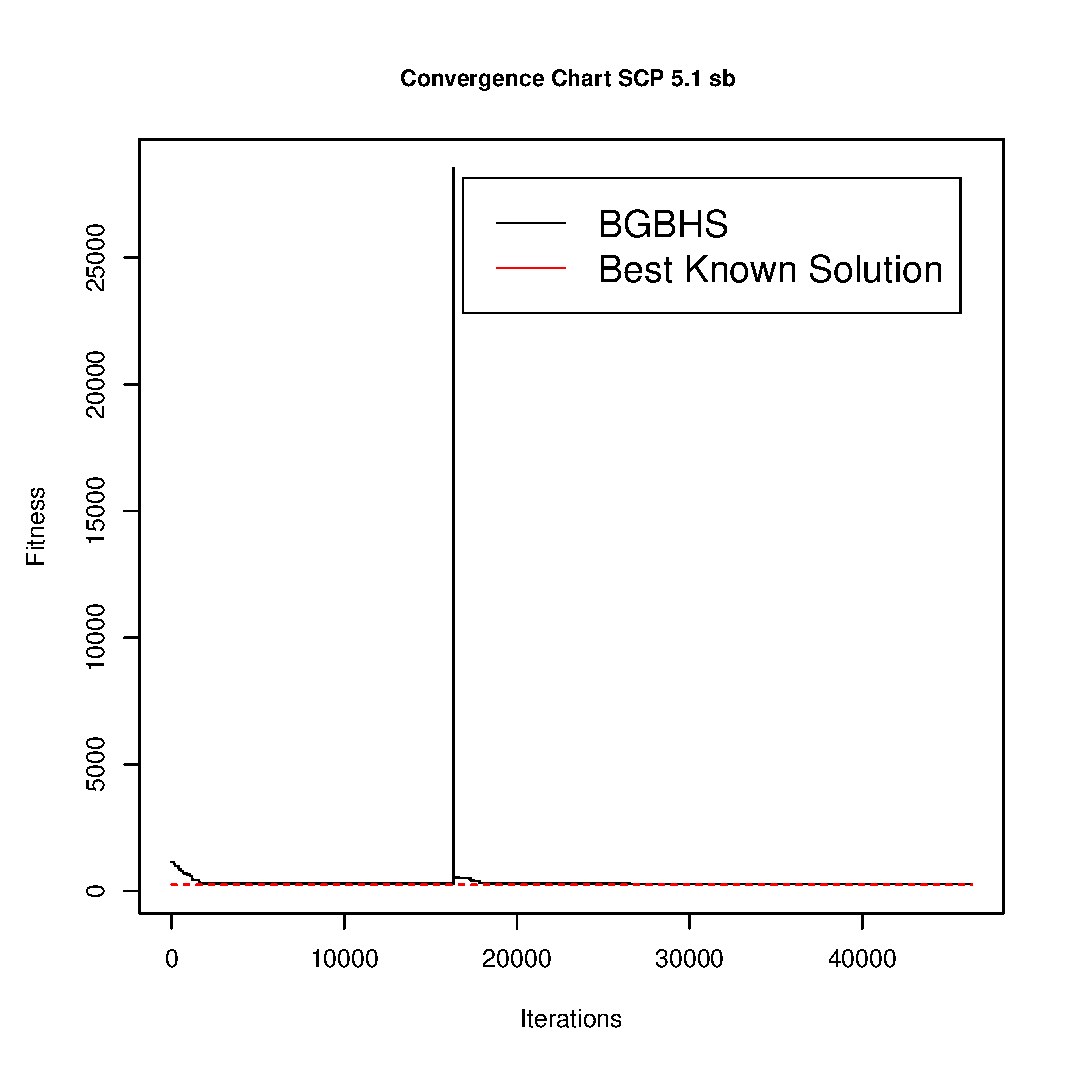
\includegraphics[width=0.45\textwidth]{Resultados/scp51_sb.eps}%
        \label{fig:b}%
        }%    
    \hfill%
    \subfloat[]{%
        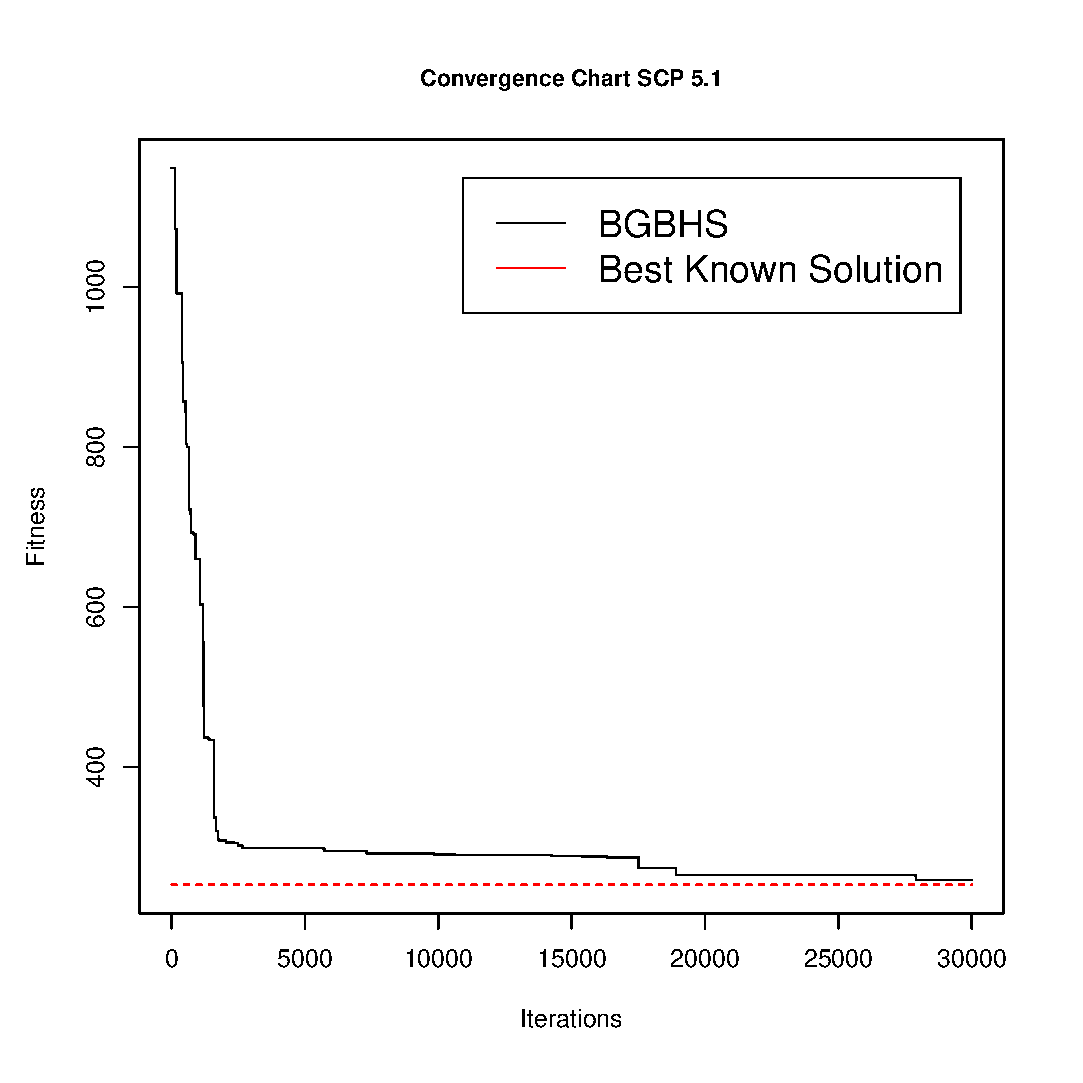
\includegraphics[width=0.45\textwidth]{Resultados/scp51.eps}%
        \label{fig:a}%
        }%
        \caption{Parameter $p$ fixed versus adaptive $p$ parameter for SCP51.}
\end{figure}


%\begin{figure}[]
%\centering
%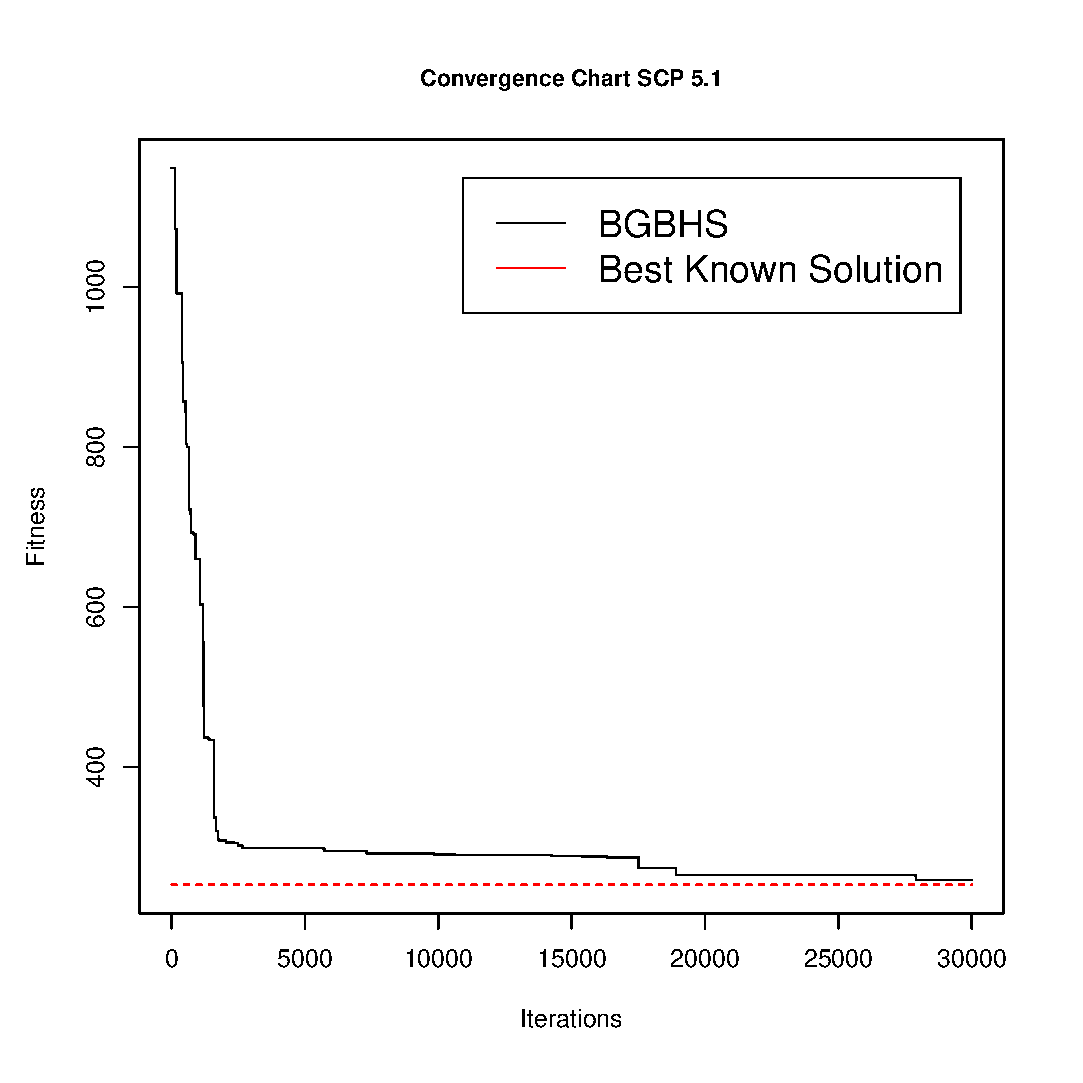
\includegraphics[scale=.45]{Resultados/scp51.eps}
%\caption{Instance 5.1.}
%\label{fig:Instance.5.1}
%\end{figure}

%---------------------------------------------SCP52
\begin{figure}[]
\centering
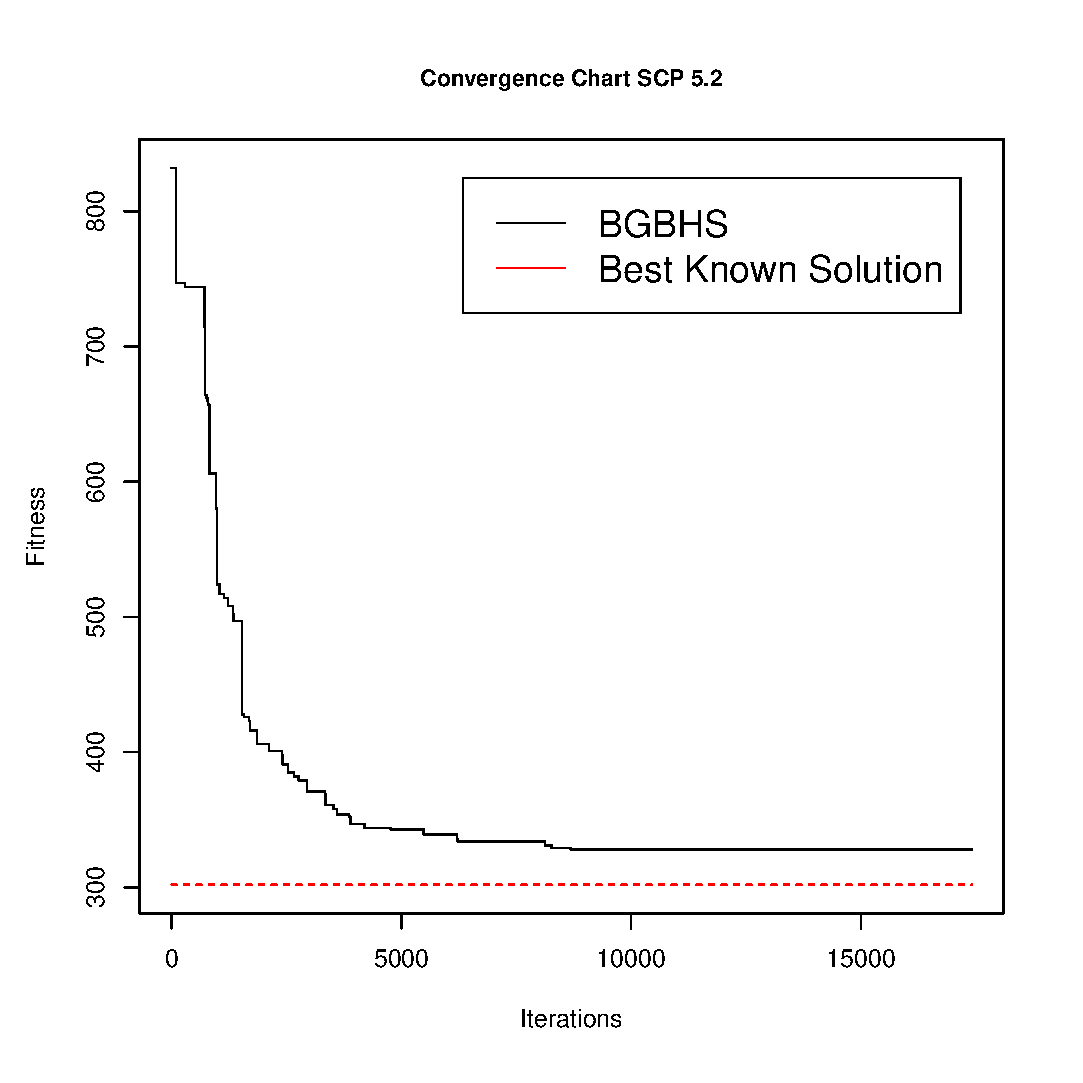
\includegraphics[scale=.45]{Resultados/scp52.eps}
\caption{Instance 5.2.}
\label{fig:Instance.5.2}
\end{figure}

%---------------------------------------------SCP53
\begin{figure}[]
\centering
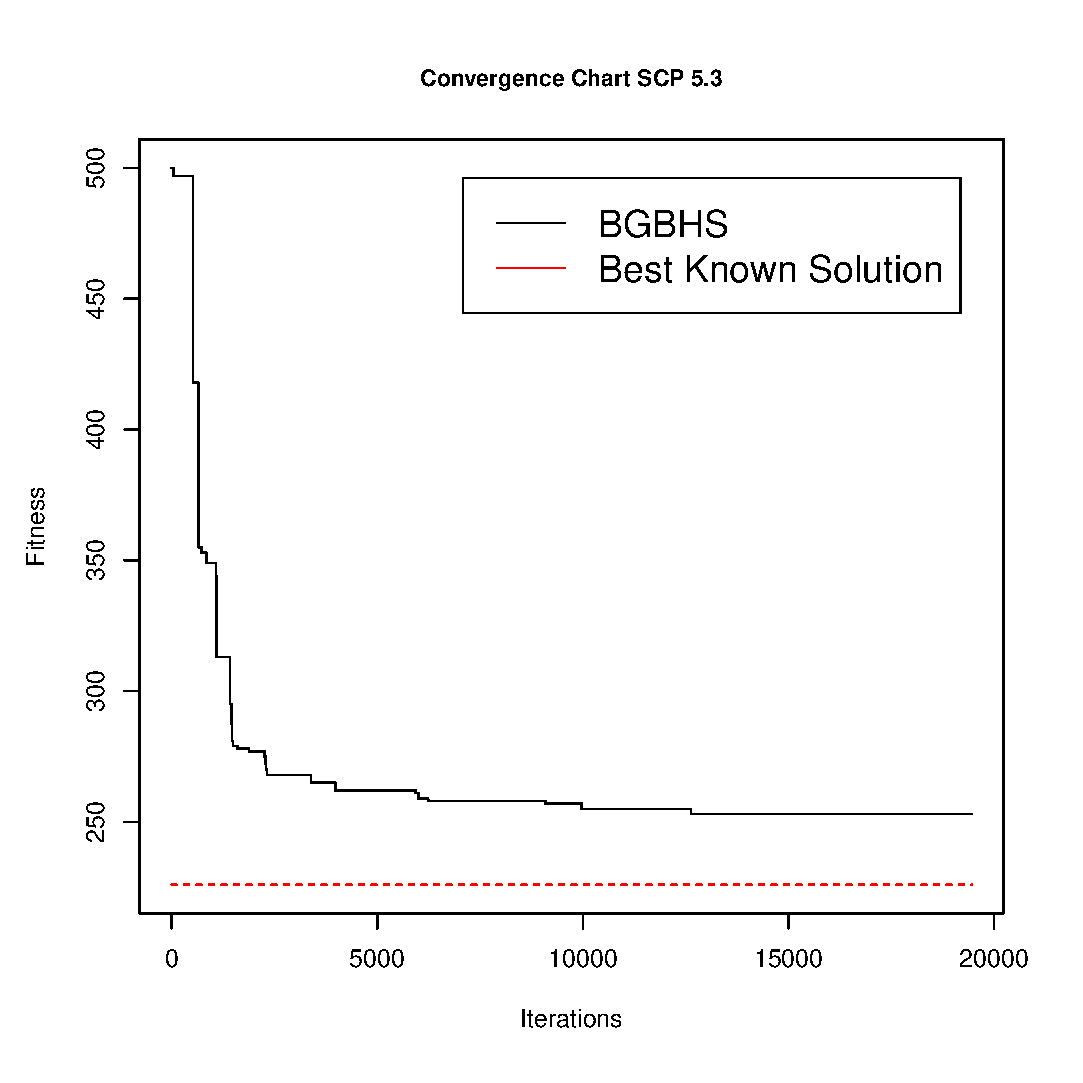
\includegraphics[scale=.45]{Resultados/scp53.eps}
\caption{Instance 5.3.}
\label{fig:Instance.5.3}
\end{figure}
%---------------------------------------------SCP54
\begin{figure}[]
\centering
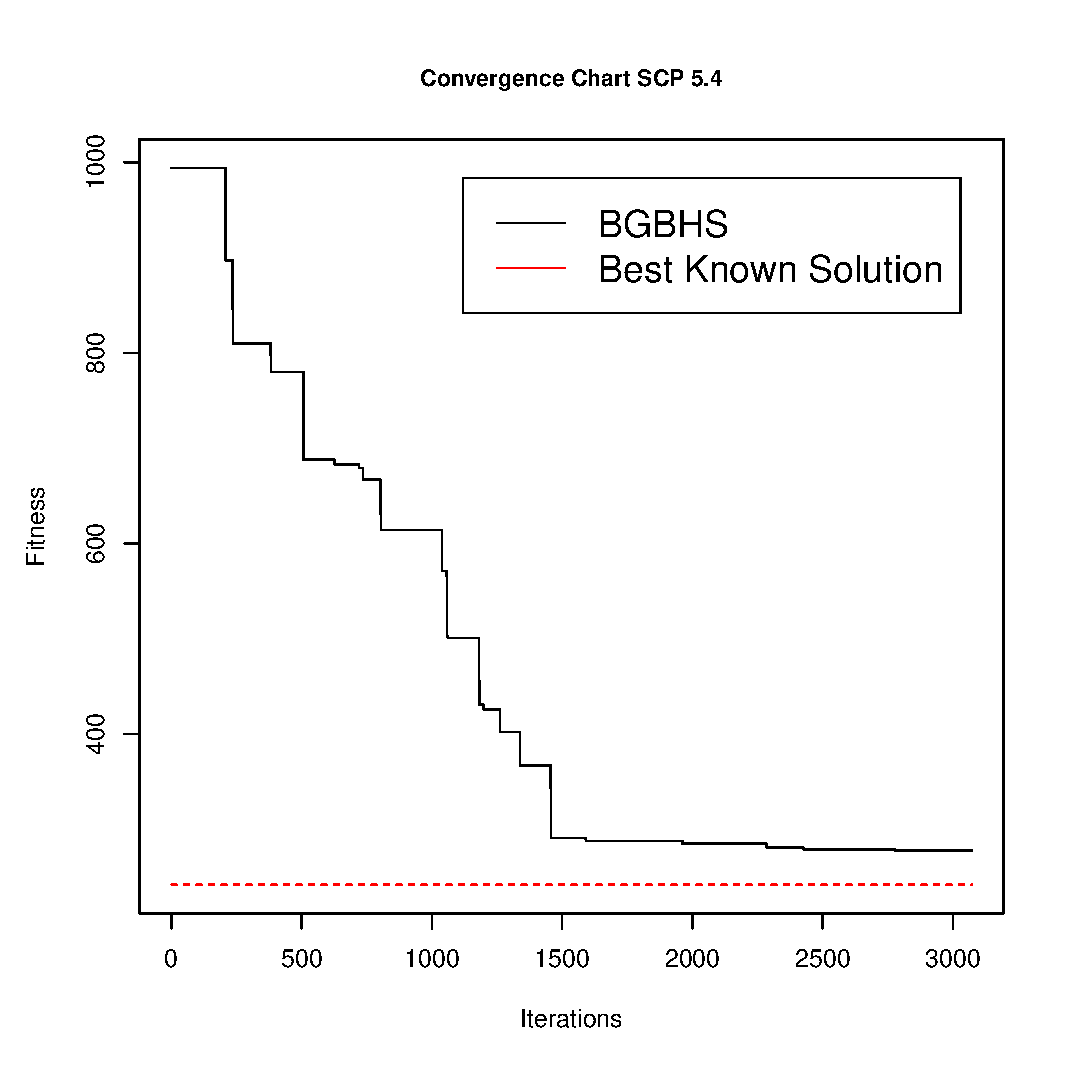
\includegraphics[scale=.45]{Resultados/scp54.eps}
\caption{Instance 5.4.}
\label{fig:Instance.5.4}
\end{figure}
%---------------------------------------------SCP55
\begin{figure}[]
\centering
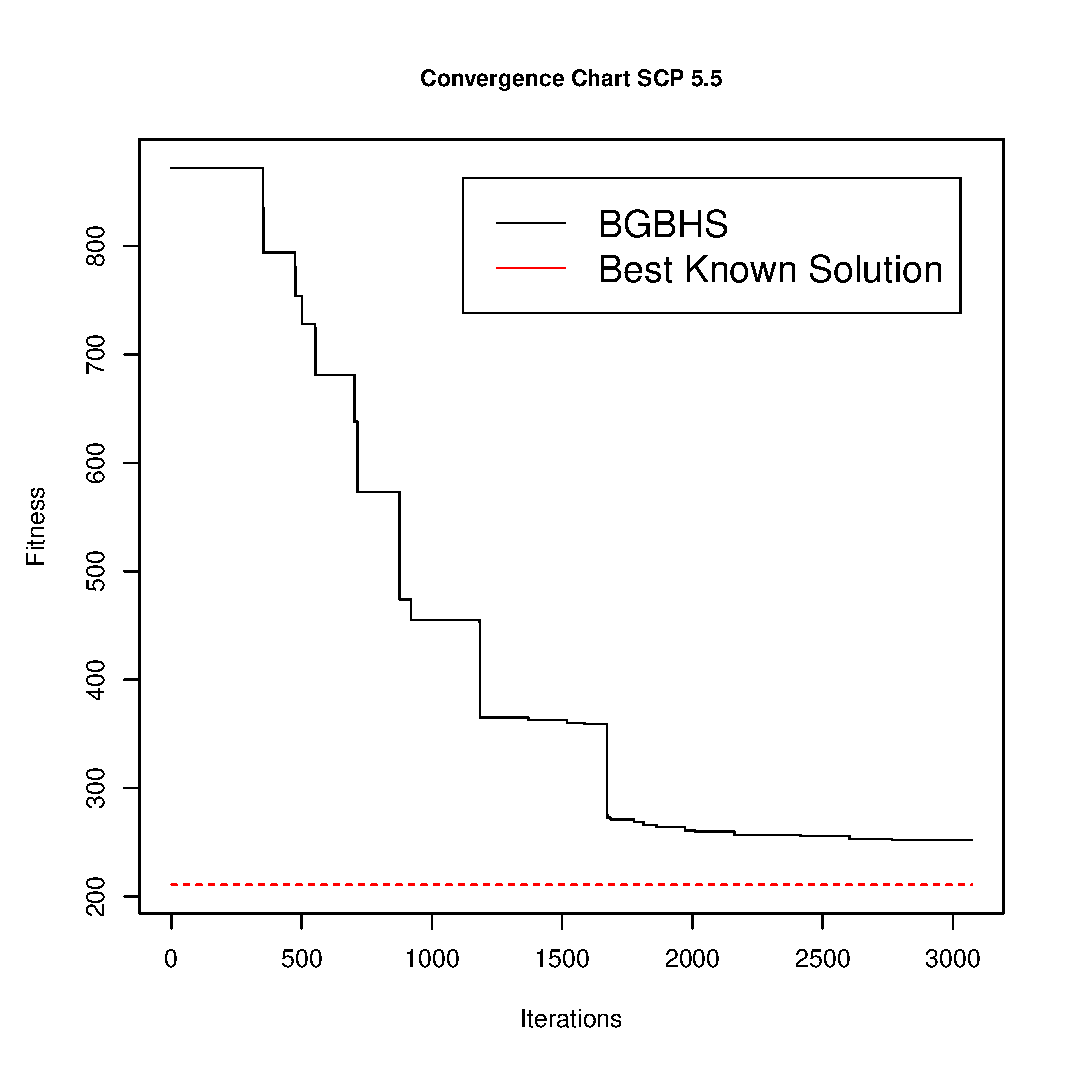
\includegraphics[scale=.45]{Resultados/scp55.eps}
\caption{Instance 5.5.}
\label{fig:Instance.5.5}
\end{figure}

%---------------------------------------------SCP56
\begin{figure}[]
\centering
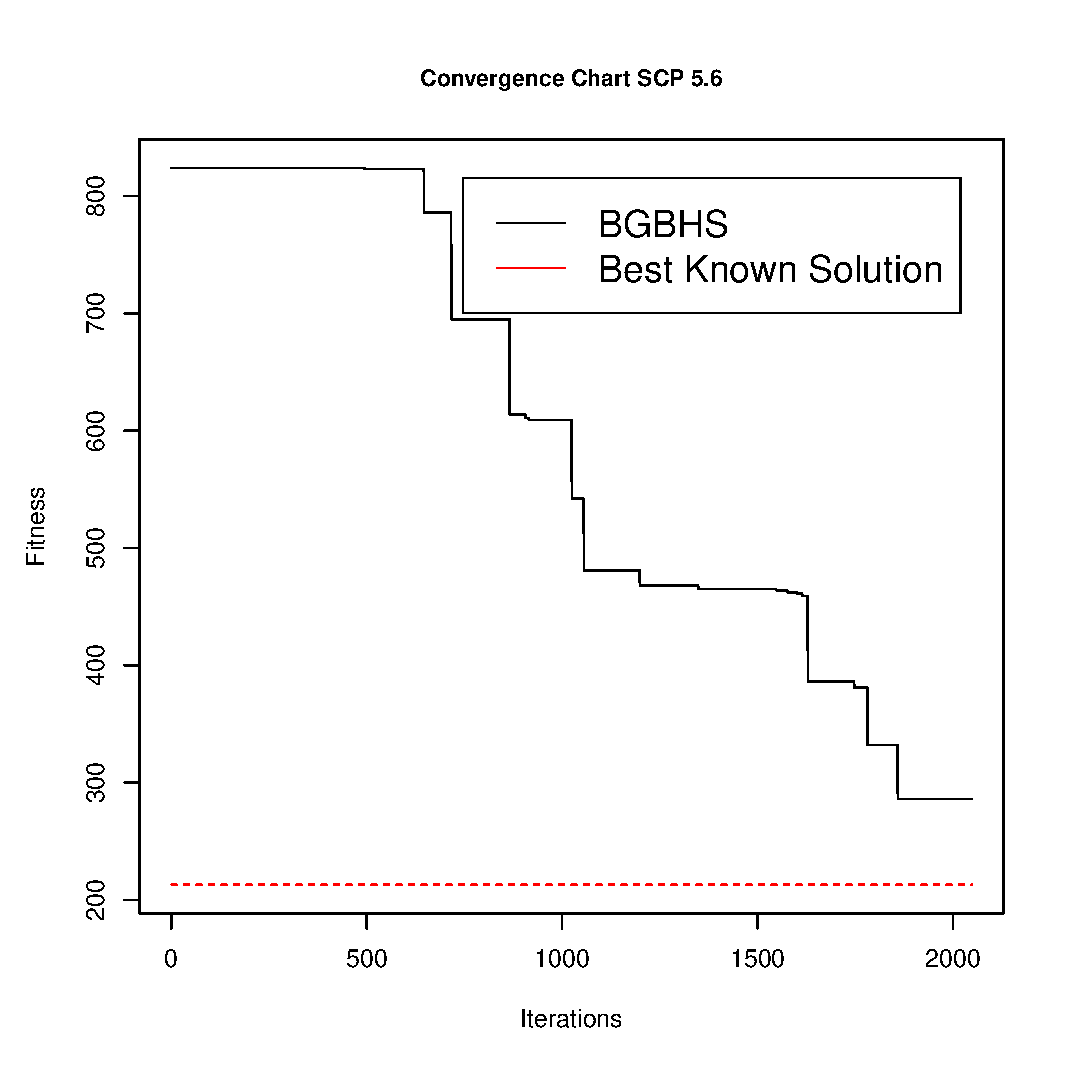
\includegraphics[scale=.45]{Resultados/scp56.eps}
\caption{Instance 5.6.}
\label{fig:Instance.5.6}
\end{figure}
%---------------------------------------------SCP57
\begin{figure}[]
\centering
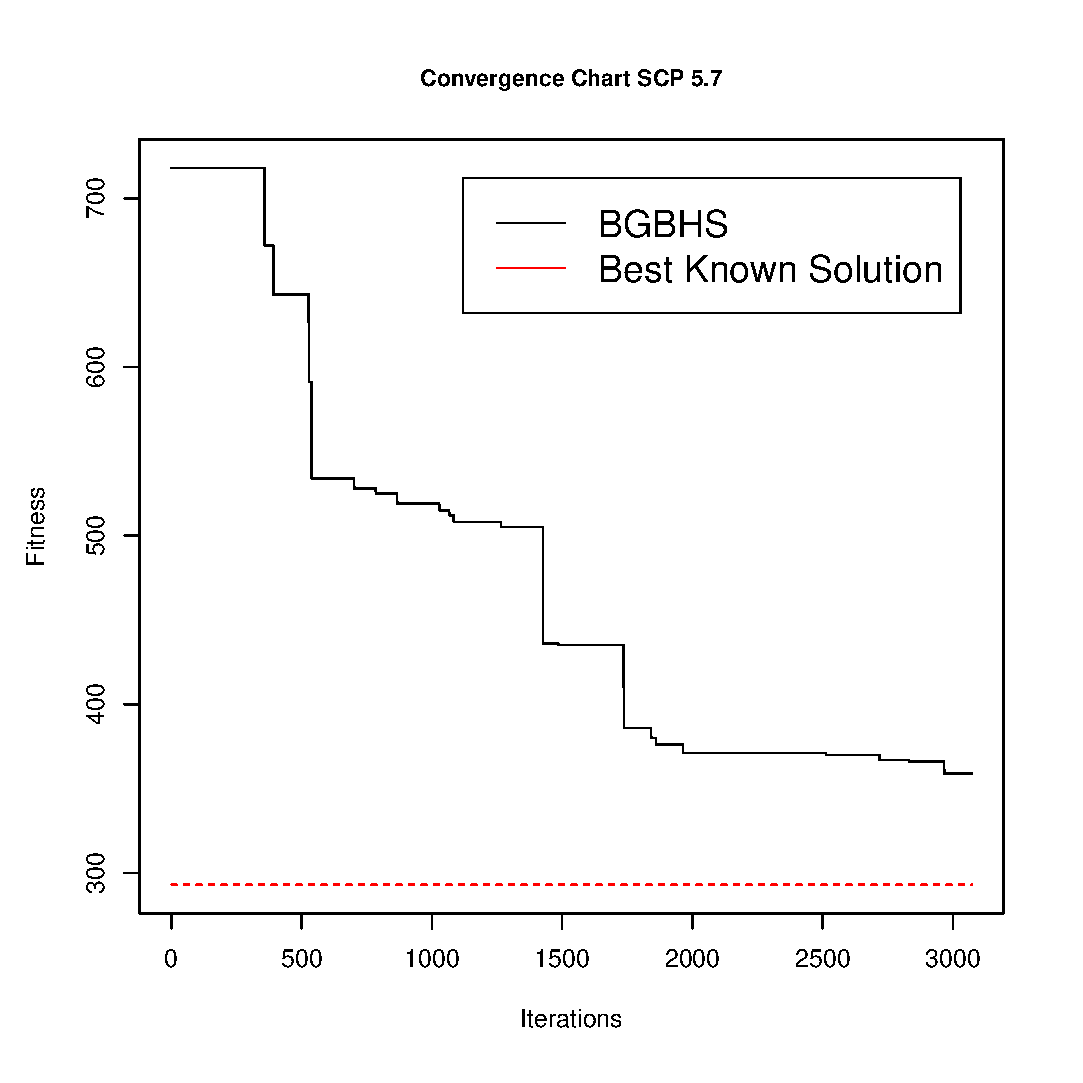
\includegraphics[scale=.45]{Resultados/scp57.eps}
\caption{Instance 5.7.}
\label{fig:Instance.5.7}
\end{figure}
%---------------------------------------------SCP58
\begin{figure}[]
\centering
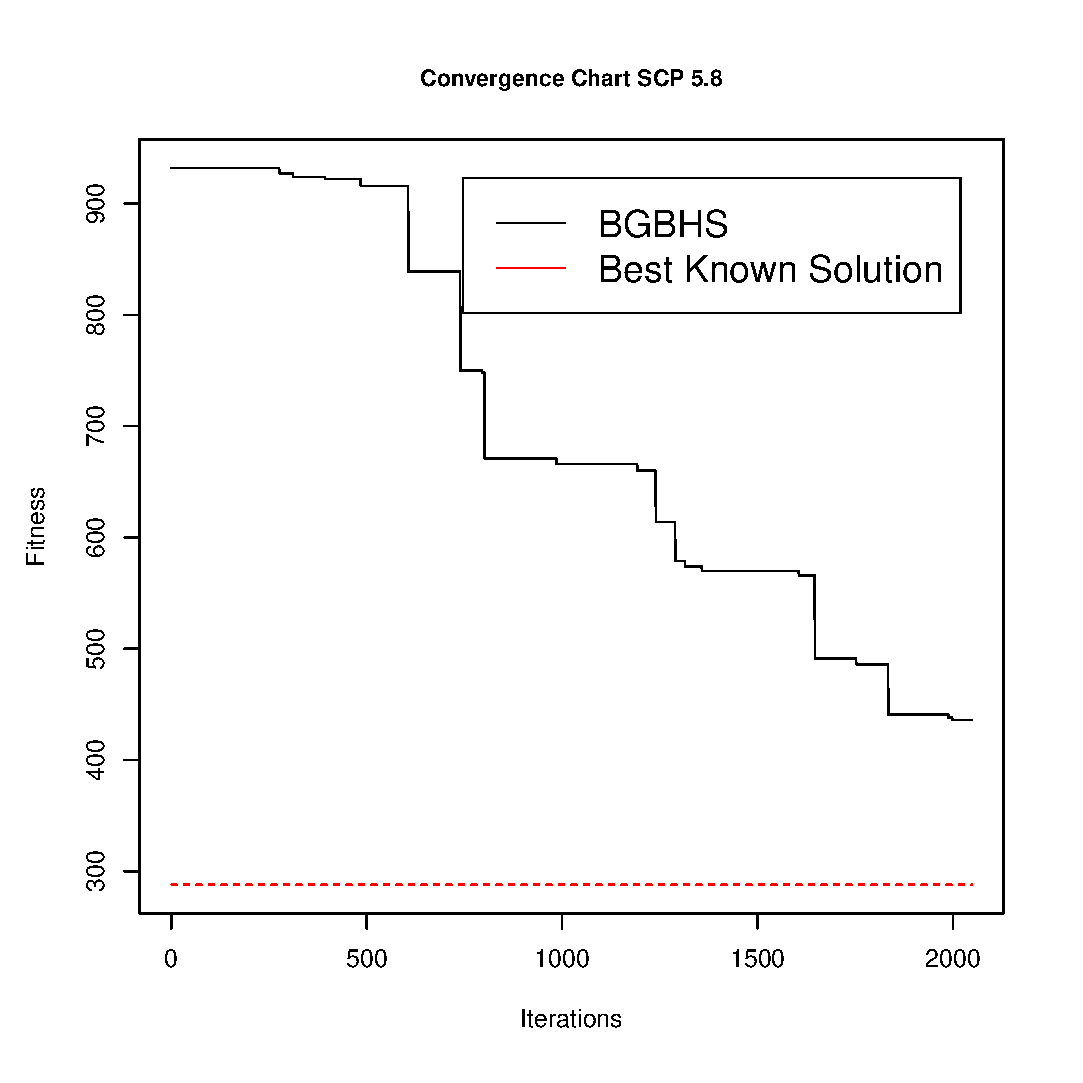
\includegraphics[scale=.45]{Resultados/scp58.eps}
\caption{Instance 5.8.}
\label{fig:Instance.5.8}
\end{figure}

%Limpieza de objetos, para liberar memoria.
\clearpage


%---------------------------------------------SCP59
\begin{figure}[]
\centering
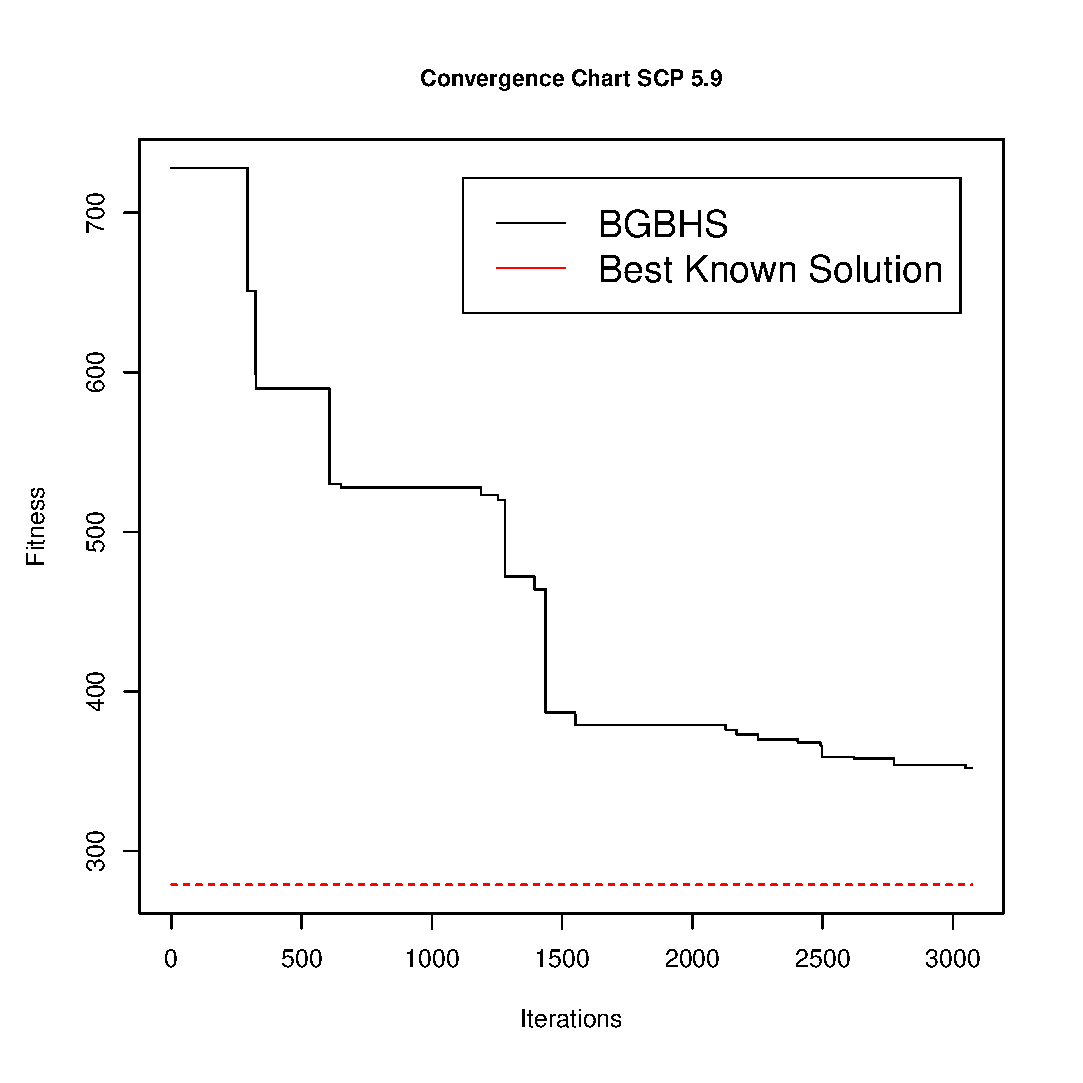
\includegraphics[scale=.45]{Resultados/scp59.eps}
\caption{Instance 5.9.}
\label{fig:Instance.5.9}
\end{figure}
%---------------------------------------------SCP510
\begin{figure}[]
\centering
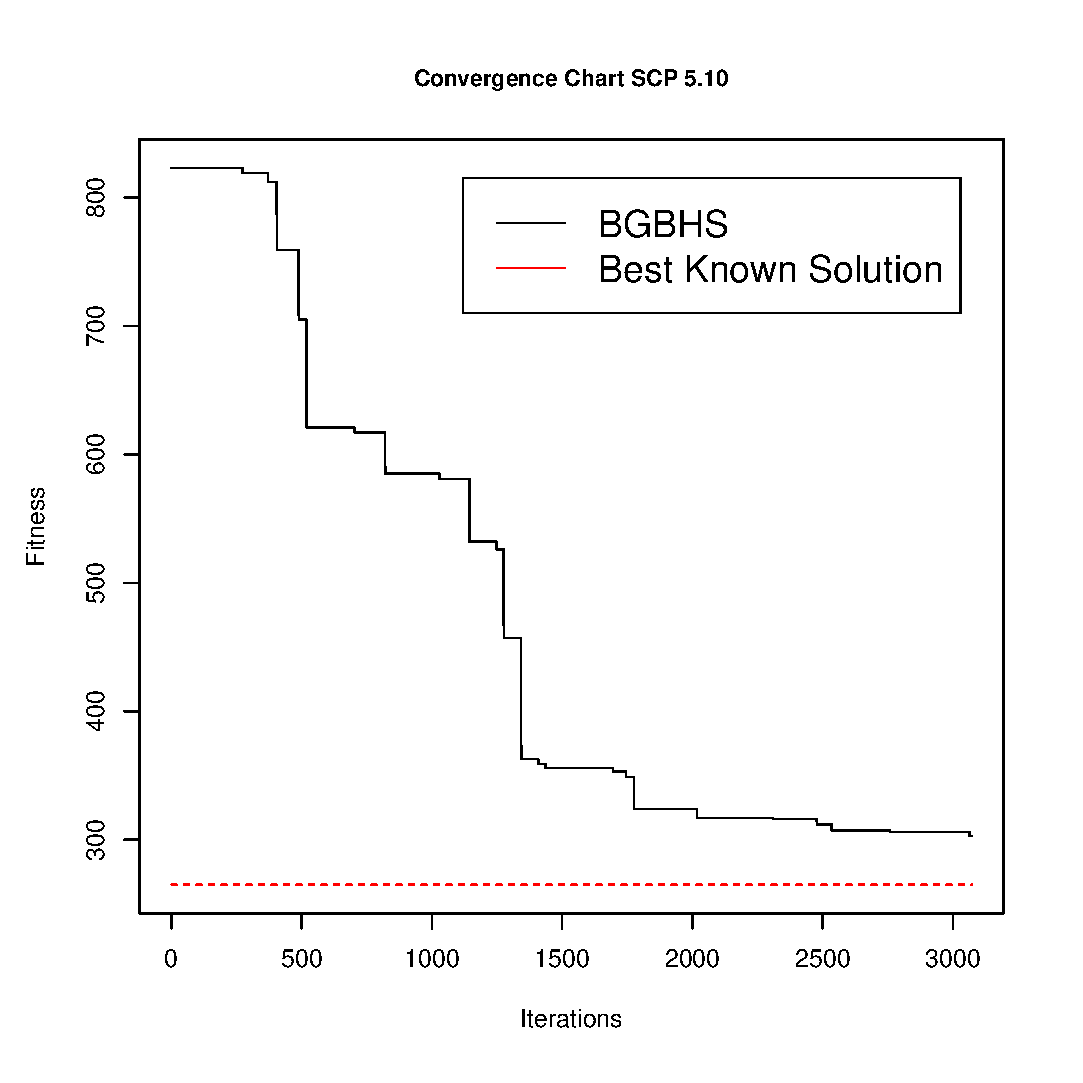
\includegraphics[scale=.45]{Resultados/scp510.eps}
\caption{Instance 5.10.}
\label{fig:Instance.5.10}
\end{figure}

%---------------------------------------------SCP61
\begin{figure}[htp] 
    \centering
    \subfloat[]{%
        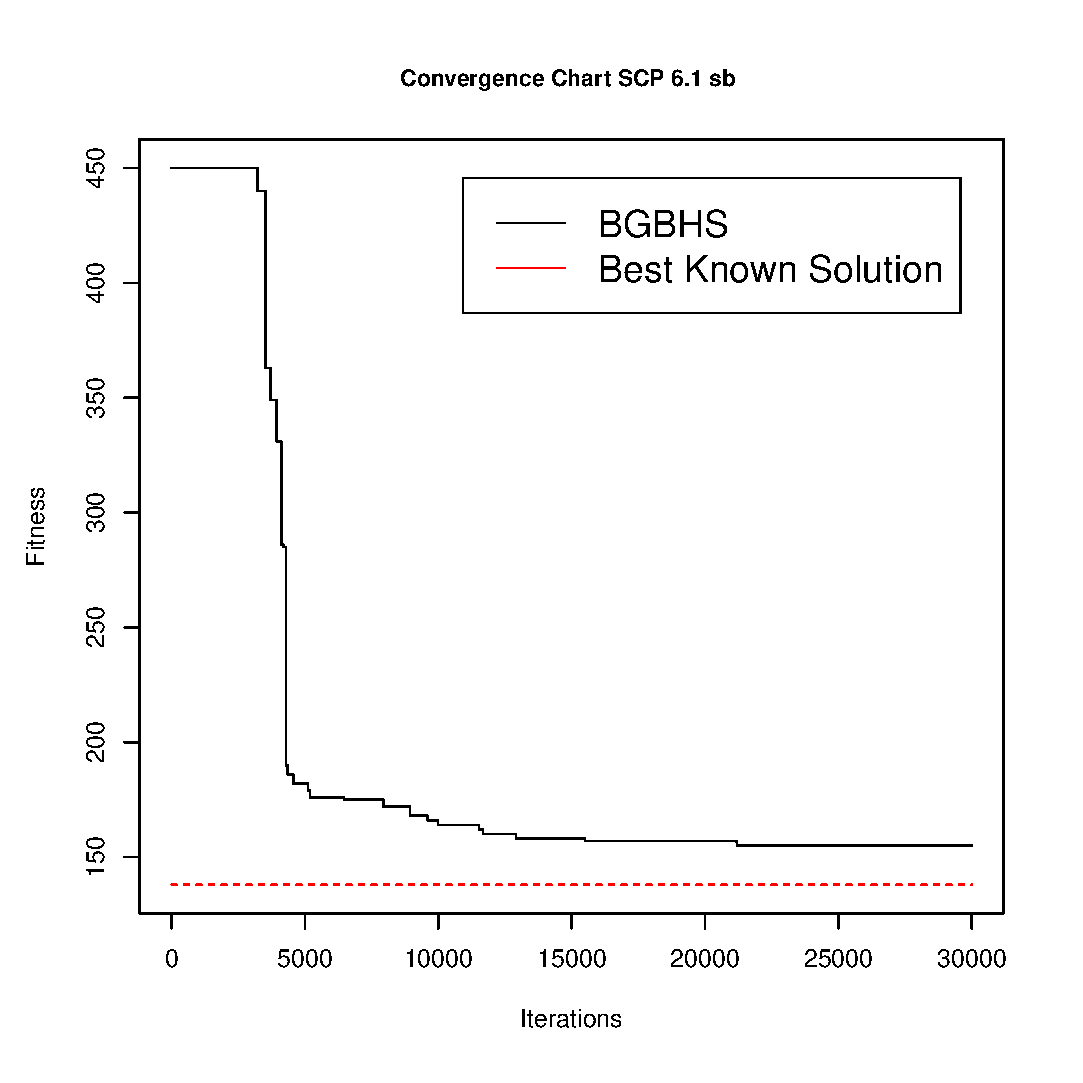
\includegraphics[width=0.45\textwidth]{Resultados/scp61_sb.eps}%
        \label{fig:b}%
        }%    
    \hfill%
    \subfloat[]{%
        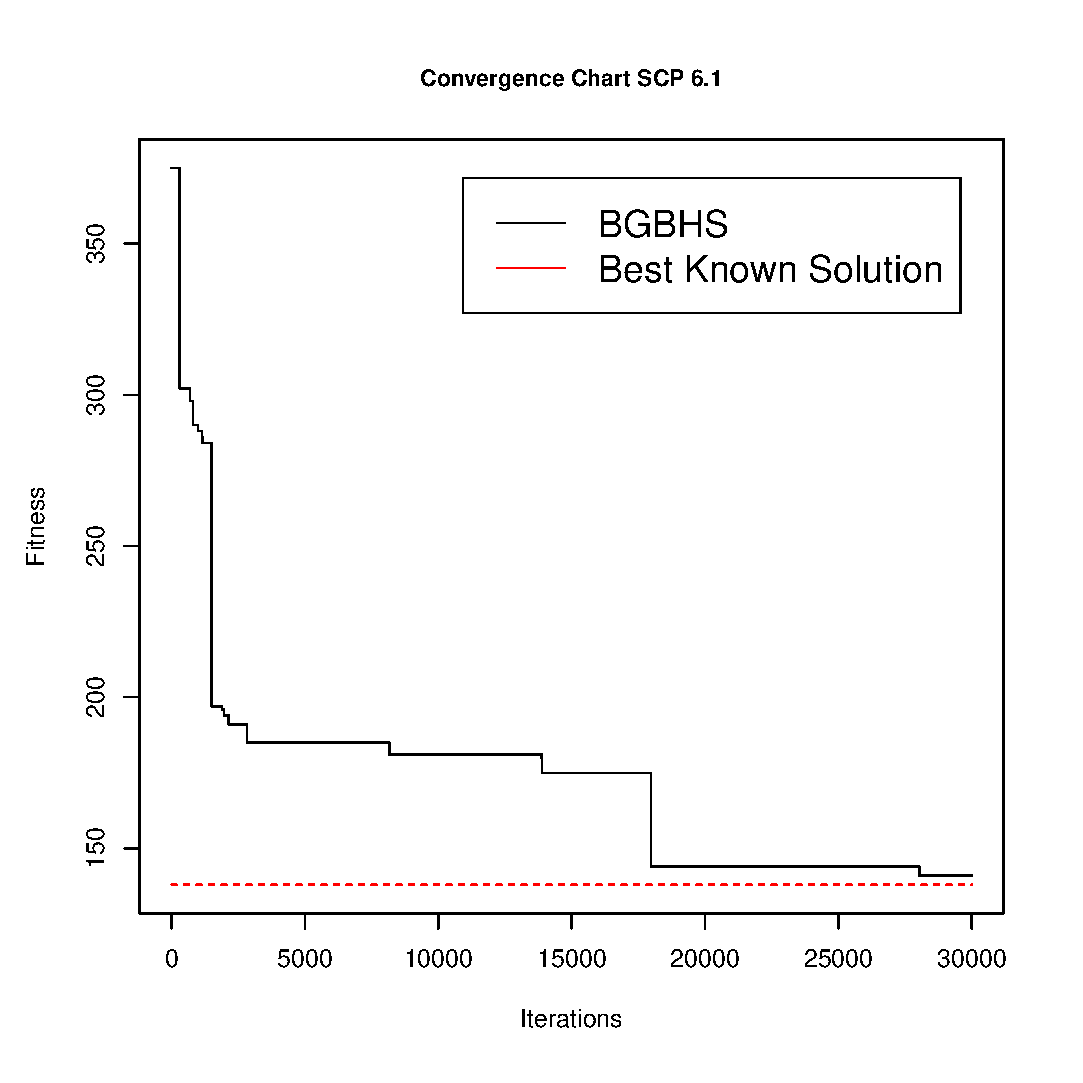
\includegraphics[width=0.45\textwidth]{Resultados/scp61.eps}%
        \label{fig:a}%
        }%
        \caption{Parameter $p$ fixed versus adaptive $p$ parameter for SCP61.}
\end{figure}

%---------------------------------------------SCP62
\begin{figure}[]
\centering
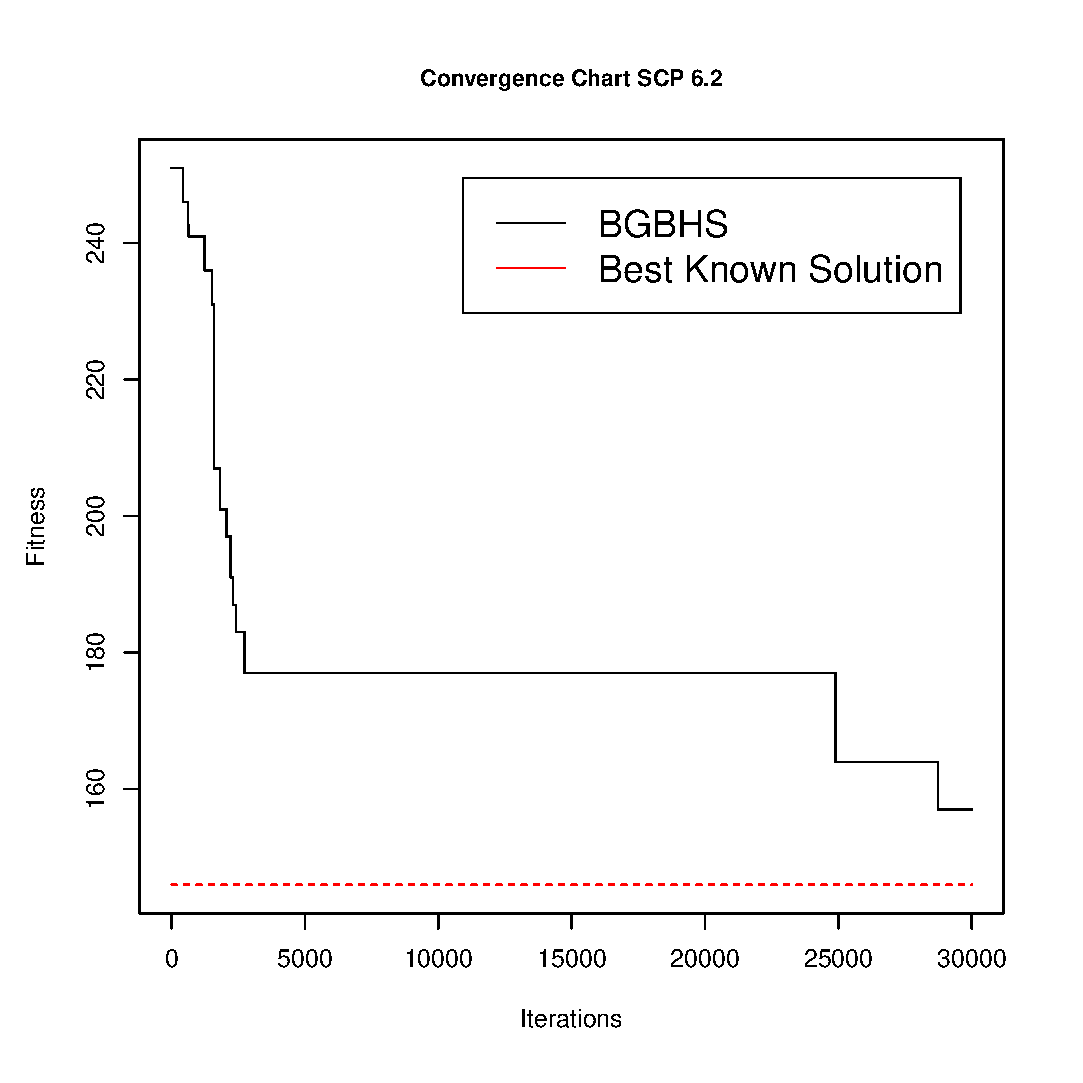
\includegraphics[scale=.45]{Resultados/scp62.eps}
\caption{Instance 6.2.}
\label{fig:Instance.6.2}
\end{figure}

%---------------------------------------------SCP63
\begin{figure}[]
\centering
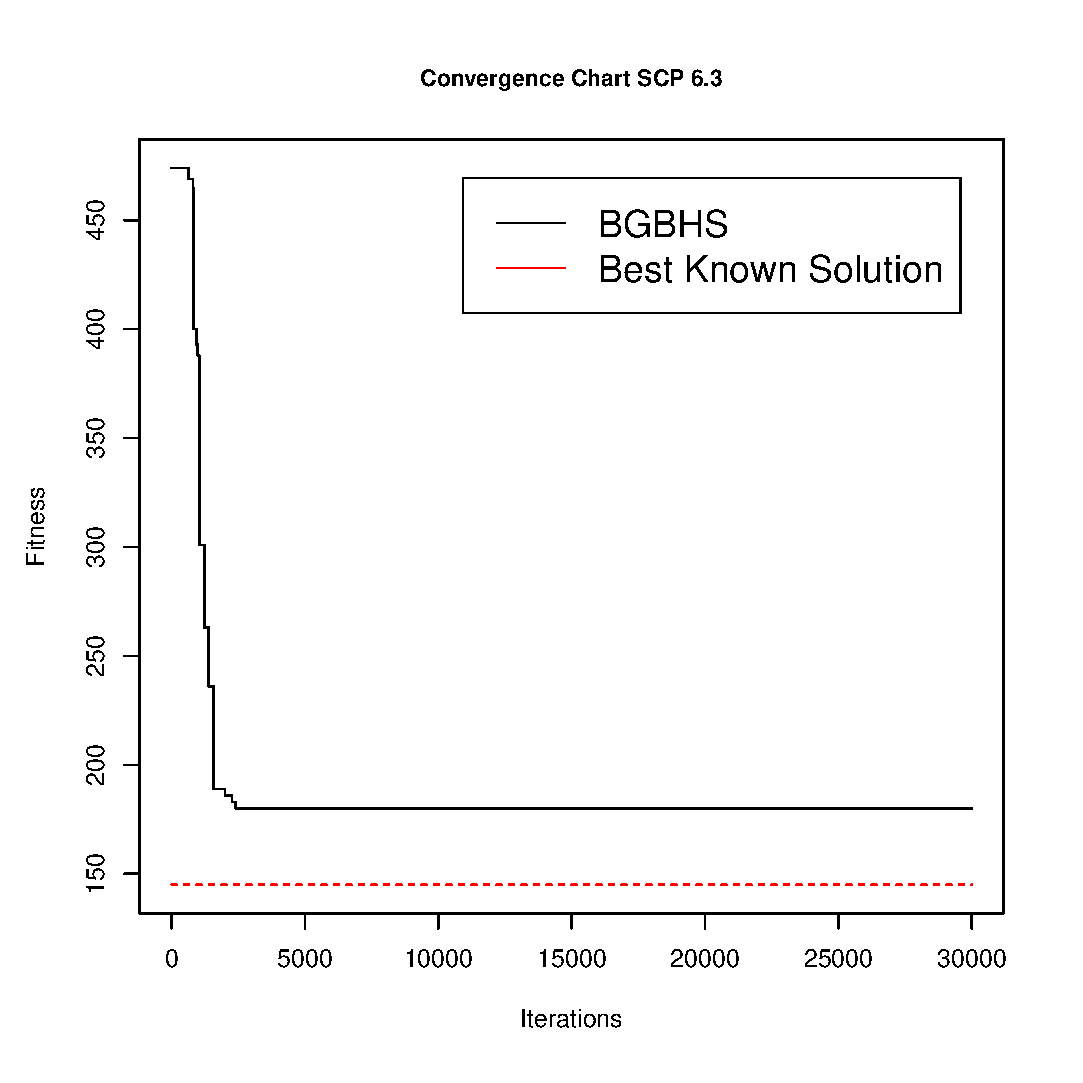
\includegraphics[scale=.45]{Resultados/scp63.eps}
\caption{Instance 6.3.}
\label{fig:Instance.6.3}
\end{figure}

%---------------------------------------------SCP64
\begin{figure}[]
\centering
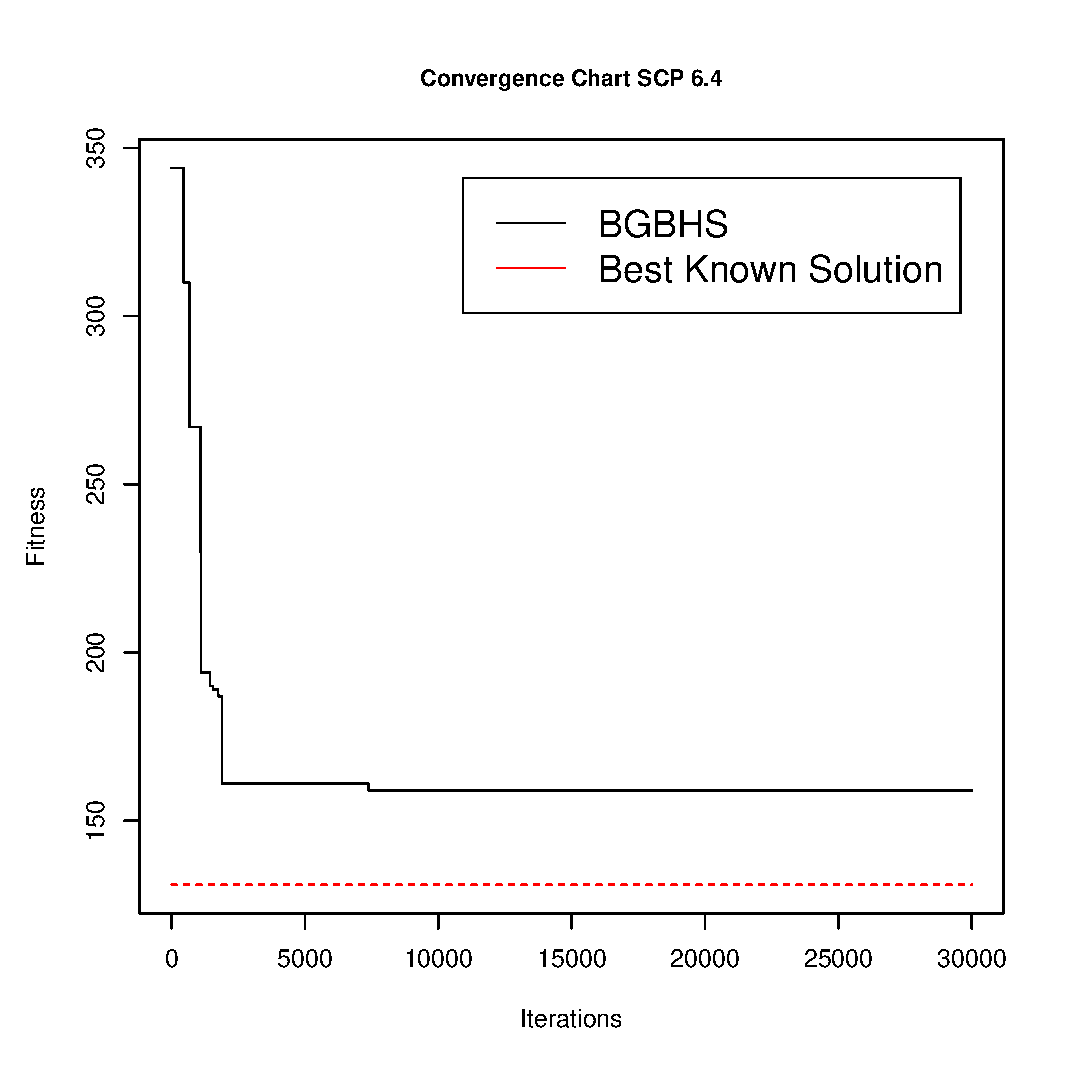
\includegraphics[scale=.45]{Resultados/scp64.eps}
\caption{Instance 6.4.}
\label{fig:Instance.6.4}
\end{figure}

%---------------------------------------------SCP65
\begin{figure}[]
\centering
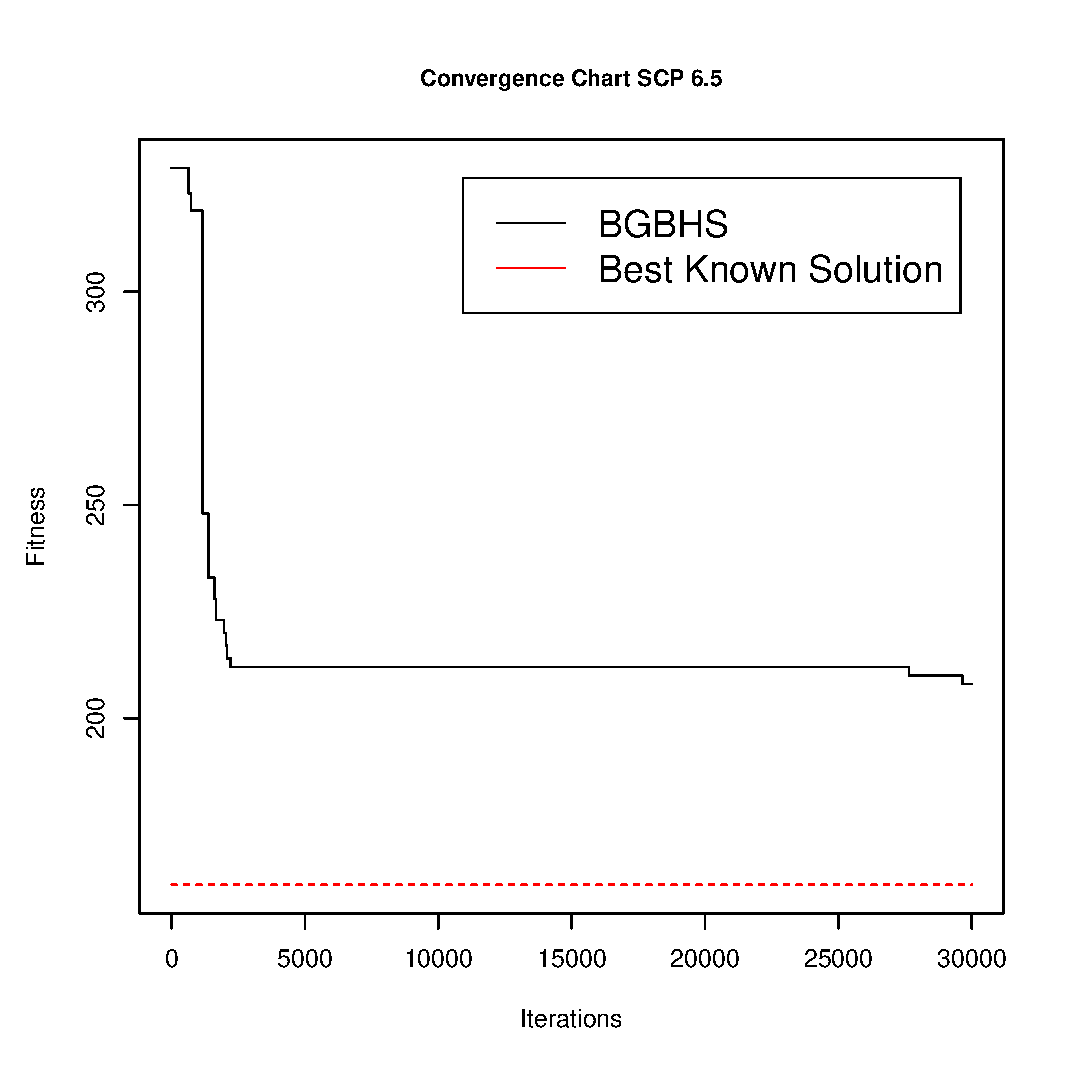
\includegraphics[scale=.45]{Resultados/scp65.eps}
\caption{Instance 6.5.}
\label{fig:Instance.6.5}
\end{figure}

%---------------------------------------------SCPA1
\begin{figure}[]
\centering
\includegraphics[scale=.45]{Resultados/scpA1.eps}
\caption{Instance A.1.}
\label{fig:Instance.A.1}
\end{figure}

%---------------------------------------------SCPA2
\begin{figure}[]
\centering
\includegraphics[scale=.45]{Resultados/scpA2.eps}
\caption{Instance A.2.}
\label{fig:Instance.A.2}
\end{figure}

%---------------------------------------------SCPA3
\begin{figure}[]
\centering
\includegraphics[scale=.45]{Resultados/scpA3.eps}
\caption{Instance A.3.}
\label{fig:Instance.A.3}
\end{figure}

%---------------------------------------------SCPA4
\begin{figure}[]
\centering
\includegraphics[scale=.45]{Resultados/scpA4.eps}
\caption{Instance A.4.}
\label{fig:Instance.A.4}
\end{figure}

%---------------------------------------------SCPA5
\begin{figure}[]
\centering
\includegraphics[scale=.45]{Resultados/scpA5.eps}
\caption{Instance A.5.}
\label{fig:Instance.A.5}
\end{figure}

%---------------------------------------------SCPB1
\begin{figure}[]
\centering
\includegraphics[scale=.45]{Resultados/scpB1.eps}
\caption{Instance B.1.}
\label{fig:Instance.B.1}
\end{figure}

%---------------------------------------------SCPB2
\begin{figure}[]
\centering
\includegraphics[scale=.45]{Resultados/scpB2.eps}
\caption{Instance B.2.}
\label{fig:Instance.B.2}
\end{figure}

%Limpieza de objetos, para liberar memoria.
\clearpage

%---------------------------------------------SCPB3
\begin{figure}[]
\centering
\includegraphics[scale=.45]{Resultados/scpB3.eps}
\caption{Instance B.3.}
\label{fig:Instance.B.3}
\end{figure}

%---------------------------------------------SCPB4
\begin{figure}[]
\centering
\includegraphics[scale=.45]{Resultados/scpB4.eps}
\caption{Instance B.4.}
\label{fig:Instance.B.4}
\end{figure}

%---------------------------------------------SCPB5
\begin{figure}[]
\centering
\includegraphics[scale=.45]{Resultados/scpB5.eps}
\caption{Instance B.5.}
\label{fig:Instance.B.5}
\end{figure}

%---------------------------------------------SCPC1
\begin{figure}[]
\centering
\includegraphics[scale=.45]{Resultados/scpC1.eps}
\caption{Instance C.1.}
\label{fig:Instance.C.1}
\end{figure}

%---------------------------------------------SCPC2
\begin{figure}[]
\centering
\includegraphics[scale=.45]{Resultados/scpC2.eps}
\caption{Instance C.2.}
\label{fig:Instance.C.2}
\end{figure}

%---------------------------------------------SCPC3
\begin{figure}[]
\centering
\includegraphics[scale=.45]{Resultados/scpC3.eps}
\caption{Instance C.3.}
\label{fig:Instance.C.3}
\end{figure}

%---------------------------------------------SCPC4
\begin{figure}[]
\centering
\includegraphics[scale=.45]{Resultados/scpC4.eps}
\caption{Instance C.4.}
\label{fig:Instance.C.4}
\end{figure}

%---------------------------------------------SCPC5
\begin{figure}[]
\centering
\includegraphics[scale=.45]{Resultados/scpC5.eps}
\caption{Instance C.5.}
\label{fig:Instance.C.5}
\end{figure}

%---------------------------------------------SCPD1
\begin{figure}[]
\centering
\includegraphics[scale=.45]{Resultados/scpD1.eps}
\caption{Instance D.1.}
\label{fig:Instance.D.1}
\end{figure}

%---------------------------------------------SCPD2
\begin{figure}[]
\centering
\includegraphics[scale=.45]{Resultados/scpD2.eps}
\caption{Instance D.2.}
\label{fig:Instance.D.2}
\end{figure}

%---------------------------------------------SCPD3
\begin{figure}[]
\centering
\includegraphics[scale=.45]{Resultados/scpD3.eps}
\caption{Instance D.3.}
\label{fig:Instance.D.3}
\end{figure}

%---------------------------------------------SCPD4
\begin{figure}[]
\centering
\includegraphics[scale=.45]{Resultados/scpD4.eps}
\caption{Instance D.4.}
\label{fig:Instance.D.4}
\end{figure}

%---------------------------------------------SCPD5
\begin{figure}[]
\centering
\includegraphics[scale=.45]{Resultados/scpD5.eps}
\caption{Instance D.5.}
\label{fig:Instance.D.5}
\end{figure}
%Instancia 4
\subsection{Instance 4.1}


\begin{table}[H]
\centering
\begin{tabular}{ | l | l | l | l | l | l | }
\hline
	Method & Optimum & Min & Max & Avg & RPD \\ \hline
	BGBHS & 429 & 534 &  &  & 24.475524475524477 \\ \hline
	BGBHS & 429 & 553 &  &  & 28.904428904428904 \\ \hline
	BGBHS & 429 & 533 &  &  & 24.242424242424242 \\ \hline
	BGBHS & 429 & 600 &  &  & 39.86013986013986 \\ \hline
	BGBHS & 429 & 438 &  &  & 2.0979020979020979 \\ \hline
	BGBHS & 429 & 460 &  &  & 7.2261072261072261 \\ \hline
	BGBHS & 429 & 455 &  &  & 6.0606060606060606 \\ \hline
	BGBHS & 429 & 470 &  &  & 9.5571095571095572 \\ \hline
	BGBHS & 429 & 533 &  &  & 24.242424242424242 \\ \hline
	BGBHS & 429 & 532 &  &  & 24.009324009324008 \\ \hline
	BGBHS IMPROVED & 429 & 451 &  &  & 5.1282051282051286 \\ \hline
	BGBHS IMPROVED & 429 & 440 &  &  & 2.5641025641025643 \\ \hline
	BGBHS IMPROVED & 429 & 460 &  &  & 7.2261072261072261 \\ \hline
	BGBHS IMPROVED & 429 & 445 &  &  & 3.7296037296037294 \\ \hline
	BGBHS IMPROVED & 429 & 470 &  &  & 9.5571095571095572 \\ \hline
	BGBHS IMPROVED & 429 & 430 &  &  & 0.23310023310023309 \\ \hline
	BGBHS IMPROVED & 429 & 430 &  &  & 0.23310023310023309 \\ \hline
	BGBHS IMPROVED & 429 & 432 &  &  & 0.69930069930069927 \\ \hline
	BGBHS IMPROVED & 429 & 435 &  &  & 1.3986013986013985 \\ \hline
	BGBHS IMPROVED & 429 & 430 &  &  & 0.23310023310023309 \\ \hline
\end{tabular}

\caption{Instance 4.1}
\label{tblscp41}
\end{table}



\newpage
\subsection{Instance 4.2}

\begin{table}[H]
\centering
\begin{tabular}{ | l | l | l | l | l | l | }
\hline
	Method & Optimum & Min & Max & Avg & RPD \\ \hline
	BGBHS & 512 & 632 &  &  & 23.4375 \\ \hline
	BGBHS & 512 & 662 &  &  & 29.296875 \\ \hline
	BGBHS & 512 & 660 &  &  & 28.90625 \\ \hline
	BGBHS & 512 & 602 &  &  & 17.578125 \\ \hline
	BGBHS & 512 & 641 &  &  & 25.1953125 \\ \hline
	BGBHS & 512 & 644 &  &  & 25.78125 \\ \hline
	BGBHS & 512 & 642 &  &  & 25.390625 \\ \hline
	BGBHS & 512 & 647 &  &  & 26.3671875 \\ \hline
	BGBHS & 512 & 641 &  &  & 25.1953125 \\ \hline
	BGBHS & 512 & 623 &  &  & 21.6796875 \\ \hline
	BGBHS IMPROVED & 512 & 550 &  &  & 7.421875 \\ \hline
	BGBHS IMPROVED & 512 & 560 &  &  & 9.375 \\ \hline
	BGBHS IMPROVED & 512 & 563 &  &  & 9.9609375 \\ \hline
	BGBHS IMPROVED & 512 & 520 &  &  & 1.5625 \\ \hline
	BGBHS IMPROVED & 512 & 523 &  &  & 2.1484375 \\ \hline
	BGBHS IMPROVED & 512 & 555 &  &  & 8.3984375 \\ \hline
	BGBHS IMPROVED & 512 & 524 &  &  & 2.34375 \\ \hline
	BGBHS IMPROVED & 512 & 518 &  &  & 1.171875 \\ \hline
	BGBHS IMPROVED & 512 & 519 &  &  & 1.3671875 \\ \hline
	BGBHS IMPROVED & 512 & 520 &  &  & 1.5625 \\ \hline
\end{tabular}
\caption{Instance 4.2}
\label{tblscp42}
\end{table}

\newpage
\subsection{Instance 4.3}
\begin{table}[H]
\centering
\begin{tabular}{ | l | l | l | l | l | l | }
\hline
	Method & Optimum & Min & Max & Avg & RPD \\ \hline
	BGBHS & 516 &  &  &  & -100 \\ \hline
	BGBHS & 516 &  &  &  & -100 \\ \hline
	BGBHS & 516 &  &  &  & -100 \\ \hline
	BGBHS & 516 &  &  &  & -100 \\ \hline
	BGBHS & 516 &  &  &  & -100 \\ \hline
	BGBHS & 516 &  &  &  & -100 \\ \hline
	BGBHS & 516 &  &  &  & -100 \\ \hline
	BGBHS & 516 &  &  &  & -100 \\ \hline
	BGBHS & 516 &  &  &  & -100 \\ \hline
	BGBHS & 516 &  &  &  & -100 \\ \hline
	BGBHS IMPROVED & 516 & 613 &  &  & 18.7984496124031 \\ \hline
	BGBHS IMPROVED & 516 &  &  &  & -100 \\ \hline
	BGBHS IMPROVED & 516 &  &  &  & -100 \\ \hline
	BGBHS IMPROVED & 516 &  &  &  & -100 \\ \hline
	BGBHS IMPROVED & 516 &  &  &  & -100 \\ \hline
	BGBHS IMPROVED & 516 &  &  &  & -100 \\ \hline
	BGBHS IMPROVED & 516 &  &  &  & -100 \\ \hline
	BGBHS IMPROVED & 516 &  &  &  & -100 \\ \hline
	BGBHS IMPROVED & 516 &  &  &  & -100 \\ \hline
	BGBHS IMPROVED & 516 &  &  &  & -100 \\ \hline
\end{tabular}

\caption{Instance 4.3}
\label{tblscp43}
\end{table}
\newpage

\subsection{Instance 4.4}
\begin{table}[H]
\centering
\begin{tabular}{ | l | l | l | l | l | l | }
\hline
	Method & Optimum & Min & Max & Avg & RPD \\ \hline
	BGBHS & 494 &  &  &  & -100 \\ \hline
	BGBHS & 494 &  &  &  & -100 \\ \hline
	BGBHS & 494 &  &  &  & -100 \\ \hline
	BGBHS & 494 &  &  &  & -100 \\ \hline
	BGBHS & 494 &  &  &  & -100 \\ \hline
	BGBHS & 494 &  &  &  & -100 \\ \hline
	BGBHS & 494 &  &  &  & -100 \\ \hline
	BGBHS & 494 &  &  &  & -100 \\ \hline
	BGBHS & 494 &  &  &  & -100 \\ \hline
	BGBHS & 494 &  &  &  & -100 \\ \hline
	BGBHS IMPROVED & 494 &  &  &  & -100 \\ \hline
	BGBHS IMPROVED & 494 &  &  &  & -100 \\ \hline
	BGBHS IMPROVED & 494 &  &  &  & -100 \\ \hline
	BGBHS IMPROVED & 494 &  &  &  & -100 \\ \hline
	BGBHS IMPROVED & 494 &  &  &  & -100 \\ \hline
	BGBHS IMPROVED & 494 &  &  &  & -100 \\ \hline
	BGBHS IMPROVED & 494 &  &  &  & -100 \\ \hline
	BGBHS IMPROVED & 494 &  &  &  & -100 \\ \hline
	BGBHS IMPROVED & 494 &  &  &  & -100 \\ \hline
	BGBHS IMPROVED & 494 &  &  &  & -100 \\ \hline
\end{tabular}

\caption{Instance 4.4}
\label{tblscp44}
\end{table}
\newpage

\subsection{Instance 4.5}
\begin{table}[H]
\centering
\begin{tabular}{ | l | l | l | l | l | l | }
\hline
	Method & Optimum & Min & Max & Avg & RPD \\ \hline
	BGBHS & 512 &  &  &  & -100 \\ \hline
	BGBHS & 512 &  &  &  & -100 \\ \hline
	BGBHS & 512 &  &  &  & -100 \\ \hline
	BGBHS & 512 &  &  &  & -100 \\ \hline
	BGBHS & 512 &  &  &  & -100 \\ \hline
	BGBHS & 512 &  &  &  & -100 \\ \hline
	BGBHS & 512 &  &  &  & -100 \\ \hline
	BGBHS & 512 &  &  &  & -100 \\ \hline
	BGBHS & 512 &  &  &  & -100 \\ \hline
	BGBHS & 512 &  &  &  & -100 \\ \hline
	BGBHS IMPROVED & 512 &  &  &  & -100 \\ \hline
	BGBHS IMPROVED & 512 &  &  &  & -100 \\ \hline
	BGBHS IMPROVED & 512 &  &  &  & -100 \\ \hline
	BGBHS IMPROVED & 512 &  &  &  & -100 \\ \hline
	BGBHS IMPROVED & 512 &  &  &  & -100 \\ \hline
	BGBHS IMPROVED & 512 &  &  &  & -100 \\ \hline
	BGBHS IMPROVED & 512 &  &  &  & -100 \\ \hline
	BGBHS IMPROVED & 512 &  &  &  & -100 \\ \hline
	BGBHS IMPROVED & 512 &  &  &  & -100 \\ \hline
	BGBHS IMPROVED & 512 &  &  &  & -100 \\ \hline
\end{tabular}

\caption{Instance 4.5}
\label{tblscp45}
\end{table}
\newpage

\subsection{Instance 4.6}
\begin{table}[H]
\centering
\begin{tabular}{ | l | l | l | l | l | l | }
\hline
	Method & Optimum & Min & Max & Avg & RPD \\ \hline
	BGBHS & 560 &  &  &  & -100 \\ \hline
	BGBHS & 560 &  &  &  & -100 \\ \hline
	BGBHS & 560 &  &  &  & -100 \\ \hline
	BGBHS & 560 &  &  &  & -100 \\ \hline
	BGBHS & 560 &  &  &  & -100 \\ \hline
	BGBHS & 560 &  &  &  & -100 \\ \hline
	BGBHS & 560 &  &  &  & -100 \\ \hline
	BGBHS & 560 &  &  &  & -100 \\ \hline
	BGBHS & 560 &  &  &  & -100 \\ \hline
	BGBHS & 560 &  &  &  & -100 \\ \hline
	BGBHS IMPROVED & 560 &  &  &  & -100 \\ \hline
	BGBHS IMPROVED & 560 &  &  &  & -100 \\ \hline
	BGBHS IMPROVED & 560 &  &  &  & -100 \\ \hline
	BGBHS IMPROVED & 560 &  &  &  & -100 \\ \hline
	BGBHS IMPROVED & 560 &  &  &  & -100 \\ \hline
	BGBHS IMPROVED & 560 &  &  &  & -100 \\ \hline
	BGBHS IMPROVED & 560 &  &  &  & -100 \\ \hline
	BGBHS IMPROVED & 560 &  &  &  & -100 \\ \hline
	BGBHS IMPROVED & 560 &  &  &  & -100 \\ \hline
	BGBHS IMPROVED & 560 &  &  &  & -100 \\ \hline
\end{tabular}

\caption{Instance 4.6}
\label{tblscp46}
\end{table}
\newpage

\subsection{Instance 4.7}
\begin{table}[H]
\centering
\begin{tabular}{ | l | l | l | l | l | l | }
\hline
	Method & Optimum & Min & Max & Avg & RPD \\ \hline
	BGBHS & 430 &  &  &  & -100 \\ \hline
	BGBHS & 430 &  &  &  & -100 \\ \hline
	BGBHS & 430 &  &  &  & -100 \\ \hline
	BGBHS & 430 &  &  &  & -100 \\ \hline
	BGBHS & 430 &  &  &  & -100 \\ \hline
	BGBHS & 430 &  &  &  & -100 \\ \hline
	BGBHS & 430 &  &  &  & -100 \\ \hline
	BGBHS & 430 &  &  &  & -100 \\ \hline
	BGBHS & 430 &  &  &  & -100 \\ \hline
	BGBHS & 430 &  &  &  & -100 \\ \hline
	BGBHS IMPROVED & 430 &  &  &  & -100 \\ \hline
	BGBHS IMPROVED & 430 &  &  &  & -100 \\ \hline
	BGBHS IMPROVED & 430 &  &  &  & -100 \\ \hline
	BGBHS IMPROVED & 430 &  &  &  & -100 \\ \hline
	BGBHS IMPROVED & 430 &  &  &  & -100 \\ \hline
	BGBHS IMPROVED & 430 &  &  &  & -100 \\ \hline
	BGBHS IMPROVED & 430 &  &  &  & -100 \\ \hline
	BGBHS IMPROVED & 430 &  &  &  & -100 \\ \hline
	BGBHS IMPROVED & 430 &  &  &  & -100 \\ \hline
	BGBHS IMPROVED & 430 &  &  &  & -100 \\ \hline
\end{tabular}

\caption{Instance 4.7}
\label{tblscp47}
\end{table}
\newpage

\subsection{Instance 4.8}
\begin{table}[H]
\centering
\begin{tabular}{ | l | l | l | l | l | l | }
\hline
	Method & Optimum & Min & Max & Avg & RPD \\ \hline
	BGBHS & 492 &  &  &  & -100 \\ \hline
	BGBHS & 492 &  &  &  & -100 \\ \hline
	BGBHS & 492 &  &  &  & -100 \\ \hline
	BGBHS & 492 &  &  &  & -100 \\ \hline
	BGBHS & 492 &  &  &  & -100 \\ \hline
	BGBHS & 492 &  &  &  & -100 \\ \hline
	BGBHS & 492 &  &  &  & -100 \\ \hline
	BGBHS & 492 &  &  &  & -100 \\ \hline
	BGBHS & 492 &  &  &  & -100 \\ \hline
	BGBHS & 492 &  &  &  & -100 \\ \hline
	BGBHS IMPROVED & 492 &  &  &  & -100 \\ \hline
	BGBHS IMPROVED & 492 &  &  &  & -100 \\ \hline
	BGBHS IMPROVED & 492 &  &  &  & -100 \\ \hline
	BGBHS IMPROVED & 492 &  &  &  & -100 \\ \hline
	BGBHS IMPROVED & 492 &  &  &  & -100 \\ \hline
	BGBHS IMPROVED & 492 &  &  &  & -100 \\ \hline
	BGBHS IMPROVED & 492 &  &  &  & -100 \\ \hline
	BGBHS IMPROVED & 492 &  &  &  & -100 \\ \hline
	BGBHS IMPROVED & 492 &  &  &  & -100 \\ \hline
	BGBHS IMPROVED & 492 &  &  &  & -100 \\ \hline
\end{tabular}

\caption{Instance 4.8}
\label{tblscp48}
\end{table}
\newpage

\subsection{Instance 4.9}
\begin{table}[H]
\centering
\begin{tabular}{ | l | l | l | l | l | l | }
\hline
	Method & Optimum & Min & Max & Avg & RPD \\ \hline
	BGBHS & 641 &  &  &  & -100 \\ \hline
	BGBHS & 641 &  &  &  & -100 \\ \hline
	BGBHS & 641 &  &  &  & -100 \\ \hline
	BGBHS & 641 &  &  &  & -100 \\ \hline
	BGBHS & 641 &  &  &  & -100 \\ \hline
	BGBHS & 641 &  &  &  & -100 \\ \hline
	BGBHS & 641 &  &  &  & -100 \\ \hline
	BGBHS & 641 &  &  &  & -100 \\ \hline
	BGBHS & 641 &  &  &  & -100 \\ \hline
	BGBHS & 641 &  &  &  & -100 \\ \hline
	BGBHS IMPROVED & 641 &  &  &  & -100 \\ \hline
	BGBHS IMPROVED & 641 &  &  &  & -100 \\ \hline
	BGBHS IMPROVED & 641 &  &  &  & -100 \\ \hline
	BGBHS IMPROVED & 641 &  &  &  & -100 \\ \hline
	BGBHS IMPROVED & 641 &  &  &  & -100 \\ \hline
	BGBHS IMPROVED & 641 &  &  &  & -100 \\ \hline
	BGBHS IMPROVED & 641 &  &  &  & -100 \\ \hline
	BGBHS IMPROVED & 641 &  &  &  & -100 \\ \hline
	BGBHS IMPROVED & 641 &  &  &  & -100 \\ \hline
	BGBHS IMPROVED & 641 &  &  &  & -100 \\ \hline
\end{tabular}

\caption{Instance 4.9}
\label{tblscp49}
\end{table}
\newpage

\subsection{Instance 4.10}
\begin{table}[H]
\centering

\caption{Instance 4.10}
\label{tblscp410}
\end{table}
\newpage

%Instancia 5
\subsection{Instance 5.1}
\begin{table}[H]
\centering

\caption{Instance 5.1}
\label{tblscp51}
\end{table}
\newpage

\subsection{Instance 5.2}
\begin{table}[H]
\centering

\caption{Instance 5.2}
\label{tblscp52}
\end{table}
\newpage

\subsection{Instance 5.3}
\begin{table}[H]
\centering

\caption{Instance 5.3}
\label{tblscp53}
\end{table}
\newpage

\subsection{Instance 5.4}
\begin{table}[H]
\centering

\caption{Instance 5.4}
\label{tblscp54}
\end{table}
\newpage

\subsection{Instance 5.5}
\begin{table}[H]
\centering

\caption{Instance 5.5}
\label{tblscp55}
\end{table}
\newpage

\subsection{Instance 5.6}
\begin{table}[H]
\centering

\caption{Instance 5.6}
\label{tblscp56}
\end{table}
\newpage

\subsection{Instance 5.7}
\begin{table}[H]
\centering

\caption{Instance 5.7}
\label{tblscp57}
\end{table}
\newpage

\subsection{Instance 5.8}
\begin{table}[H]
\centering

\caption{Instance 5.8}
\label{tblscp58}
\end{table}
\newpage

\subsection{Instance 5.9}
\begin{table}[H]
\centering

\caption{Instance 5.9}
\label{tblscp59}
\end{table}
\newpage

\subsection{Instance 5.10}
\begin{table}[H]
\centering

\caption{Instance 5.10}
\label{tblscp510}
\end{table}
\newpage


%Instancia 6
\subsection{Instance 6.1}
\begin{table}[H]
\centering

\caption{Instance 6.1}
\label{tblscp61}
\end{table}
\newpage

\subsection{Instance 6.2}
\begin{table}[H]
\centering

\caption{Instance 6.2}
\label{tblscp62}
\end{table}
\newpage

\subsection{Instance 6.3}
\begin{table}[H]
\centering

\caption{Instance 6.3}
\label{tblscp63}
\end{table}
\newpage

\subsection{Instance 6.4}
\begin{table}[H]
\centering

\caption{Instance 6.4}
\label{tblscp64}
\end{table}
\newpage

\subsection{Instance 6.5}
\begin{table}[H]
\centering

\caption{Instance 6.5}
\label{tblscp65}
\end{table}
\newpage

%Instancia A
\subsection{Instance A.1}
\begin{table}[H]
\centering

\caption{Instance A.1}
\label{tblscpA1}
\end{table}

\newpage

\subsection{Instance A.2}
\begin{table}[H]
\centering

\caption{Instance A.2}
\label{tblscpA2}
\end{table}

\newpage
\subsection{Instance A.3}
\begin{table}[H]
\centering

\caption{Instance A.3}
\label{tblscpA3}
\end{table}

\newpage
\subsection{Instance A.4}
\begin{table}[H]
\centering

\caption{Instance A.3}
\label{tblscpA3}
\end{table}

\newpage
\subsection{Instance A.5}
\begin{table}[H]
\centering

\caption{Instance A.5}
\label{tblscpA5}
\end{table}

\newpage

%Instancia B
\subsection{Instance B.1}
\begin{table}[H]
\centering

\caption{Instance B.1}
\label{tblscpB1}
\end{table}

\newpage
\subsection{Instance B.2}
\begin{table}[H]
\centering

\caption{Instance B.2}
\label{tblscpB2}
\end{table}
\newpage

\subsection{Instance B.3}
\begin{table}[H]
\centering

\caption{Instance B.3}
\label{tblscpB3}
\end{table}
\newpage

\subsection{Instance B.4}
\begin{table}[H]
\centering

\caption{Instance B.4}
\label{tblscpB4}
\end{table}
\newpage

\subsection{Instance B.5}
\begin{table}[H]
\centering

\caption{Instance B.5}
\label{tblscpB5}
\end{table}
\newpage

%Instancia C
\subsection{Instance C.1}
\begin{table}[H]
\centering

\caption{Instance C.1}
\label{tblscpC1}
\end{table}
\newpage
\subsection{Instance C.2}
\begin{table}[H]
\centering

\caption{Instance C.2}
\label{tblscpC2}
\end{table}
\newpage

\subsection{Instance C.3}
\begin{table}[H]
\centering

\caption{Instance C.3}
\label{tblscpC3}
\end{table}
\newpage

\subsection{Instance C.4}
\begin{table}[H]
\centering

\caption{Instance C.4}
\label{tblscpC4}
\end{table}
\newpage

\subsection{Instance C.5}
\begin{table}[H]
\centering

\caption{Instance C.5}
\label{tblscpC5}
\end{table}
\newpage

%Instancia D
\subsection{Instance D.1}
\begin{table}[H]
\centering

\caption{Instance D.1}
\label{tblscpD1}
\end{table}
\newpage

\subsection{Instance D.2}
\begin{table}[H]
\centering

\caption{Instance D.2}
\label{tblscpD2}
\end{table}
\newpage

\subsection{Instance D.3}
\begin{table}[H]
\centering

\caption{Instance D.3}
\label{tblscpD3}
\end{table}
\newpage

\subsection{Instance D.4}
\begin{table}[H]
\centering

\caption{Instance D.4}
\label{tblscpD4}
\end{table}
\newpage

\subsection{Instance D.5}
\begin{table}[H]
\centering

\caption{Instance D.5}
\label{tblscpD5}
\end{table}
\newpage


